%importation des packages
\RequirePackage{pdfmanagement-testphase}
\DocumentMetadata {lang=fr}
\documentclass[fontsize=11pt,twoside=true,DIV=calc,parskip=half]{scrbook}
\usepackage{scrhack}
\usepackage{scrlayer-scrpage} %équivalent de fancyhdr pour kommascript
\usepackage[french]{babel}
\usepackage{fancyref}
\usepackage[autostyle=true]{csquotes} % csquotes va utiliser la langue définie dans babel
\usepackage[shortlabels]{enumitem} %permet de faire \begin{enumerate}[a)]
\usepackage{tabularx}
\usepackage{amsmath} %formules mathématiques
\usepackage{amssymb} %symboles mathématiques
\usepackage{amsfonts} %polices mathématiques

%Loading xcolor with dvipsnames
\usepackage[dvipsnames]{xcolor}
%\usepackage{anyfontsize}
%\usepackage{graphicx}
%\usepackage{wrapfig}%image à doite ou a gauche du texte
\usepackage{svg}
\usepackage{tikz}
\usetikzlibrary{optics}
\usepackage{tkz-base}
\usepackage{tkz-fct}
\usepackage{tkz-euclide}
\usepackage{multido}%pour la macro pointillés
\usepackage[breakable]{tcolorbox}
\tcbuselibrary{theorems}
\tcbuselibrary{skins,listings}
\usepackage{siunitx}
\usepackage{qrcode}


%\usepackage{pstricks}%pour dessiner les champs électriques
%\usepackage{pst-magneticfield}%pour dessiner les champs magnétiques
%\usepackage{pst-coil,pst-slpe,pstricks-add}

%hyperliens
\usepackage{hyperref}
\hypersetup{
  colorlinks,
  citecolor=black,
  filecolor=black,
  linkcolor=black,
  urlcolor=black
}

\usepackage[noabbrev]{cleveref}
%couleurs
\definecolor{LightBlue}{HTML}{ADD8E6}

%police
%\usepackage{libertine} la police libertine et T1 ne permettent pas d'afficher les smallcaps, ni les upper+bold.
\usepackage[T1]{fontenc}

%cadre
\usepackage{framed}

%graphique tikz
\usepackage{tkz-euclide}
\usepackage{tkz-fct}

%chemin vers les images
\graphicspath{ {./images/} }

%exercices xsim
\usepackage[use-files]{xsim}
\DeclareExerciseTagging{difficulty}
\xsimsetup{
  path=xsim,
  load-style = layouts ,
  exercise/template = runin ,
  solution/template = runin,
  difficulty={*,**,***},
}



%math
\everymath{\displaystyle} %pour que les équations soient bien présentées




%mise en page générale
\KOMAoptions{DIV=last}
\usepackage{setspace}%pour regler l'interligne
\onehalfspacing %interligne1.5
\setlength{\parindent}{0pt} %pas de retrait en début de paragraphe
\usepackage{caption}%mise en forme des légendes des figures
\addtokomafont{caption}{\scriptsize \slshape}
\addtokomafont{captionlabel}{\scriptsize \slshape}


%pieds de page utiliser scrlayer-scrpage
\setkomafont{pageheadfoot}{\small}
\lohead{} \rohead{} \cohead{}
\lofoot{Ondes et phénomènes périodiques - physique(2h) - 6GT}
\rofoot{Page \thepage}
\cofoot{}


%style perso et macro
\definecolor{NavyBlue}{HTML}{7279ff}
\definecolor{mygray1}{HTML}{e7e7e7}%light
\definecolor{mygray2}{HTML}{676767}%lightdark
\definecolor{Green}{HTML}{1d8600}%poleS
\definecolor{BrickRed}{HTML}{b30003}%poleN
\definecolor{Weiss}{rgb}{1,0.98,0.98}%  255 250 250 %main droite
\definecolor{Haut}{rgb}{1,0.894,0.769}% 255 228 196 %main droite
\definecolor{Auge}{rgb}{0.54,0.27,0.074}% 139 69 19 %main droite
\newcommand{\motcle}[1]{
  \uppercase{\textbf{#1}}
}

\newcommand{\pointilles}[1]{
  \begin{itemize}[label={}]
    \multido{}{#1}{\item \dotfill}
  \end{itemize}
}

\newenvironment{encadre}{\begin{center}\begin{minipage}[c]{0.8\linewidth}\begin{tcolorbox}}{\end{tcolorbox}\end{minipage}\end{center}}






%les variables du document
\subject{Physique(2h)}
\title{\Huge{Ondes et phénomènes périodiques}}
\subtitle{6\textsuperscript{ème} GT}
\author {J.N. Gautier}
\date{}

\begin{document}
\maketitle
\chapter{Les phénomènes périodiques}
La révolution de la Terre, un enfant sur une balançoire, une roue qui tourne, les battements du c\oe{}ur, \ldots de nombreux phénomènes du quotidien se répètent toujours de la même manière, ils présentent un \motcle{caractère périodique}.

Parmi les phénomènes périodiques, certains consistent en un va-et-vient autour d'une position d'équilibre : la balançoire, une latte qui vibre au bord d'un bureau, un ressort avec une masse à son extrémité, ce sont des phénomènes d'\motcle{oscillation}.
\begin{figure}[h!]
    \begin{minipage}{.5\textwidth}
        \centering
        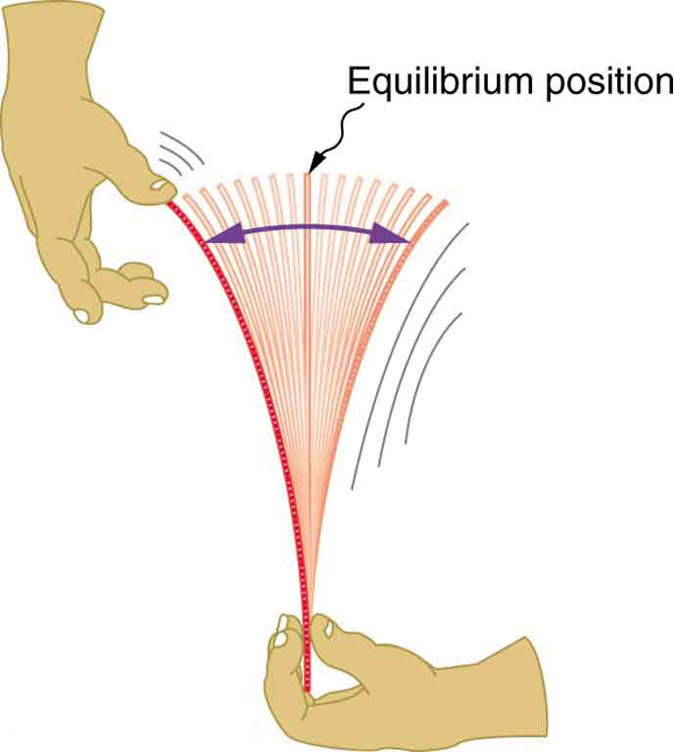
\includegraphics[width=.8 \linewidth]{latte_vibre.png}
        %\includesvg[inkscapelatex=false, width=.5 \linewidth]{tir_oblique.svg}
        \caption{Une tige rigide vibrant par rapport à sa position de repos est un oscillateur.}
        \label{lame_vibre}
    \end{minipage}
    \begin{minipage}{.5\textwidth}
        \centering
        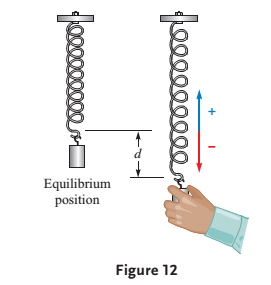
\includegraphics[width=.8 \linewidth]{ressort_oscille.png}
        \caption{Une masse attachée à un ressort est un exemple très classique d'oscillateur.}
        \label{lame_vibre_2}
    \end{minipage}
\end{figure}

\newpage

\section{Caractéristiques des oscillateurs}
Lorsqu'on cherche à étudier un phénomène, il est indispensable de prendre conscience des paramètres qui le caractérise afin de pouvoir mesurer ceux-ci.
Après avoir observé le pendule qui oscille, précise quels sont les paramètres caractéristiques des phénomènes d'oscillation.
\begin{itemize}[label=\textbullet]
    \item Élongation : \dotfill
          \pointilles{2}
    \item Amplitude : \dotfill
          \pointilles{2}
    \item Fréquence : \dotfill
          \pointilles{2}
    \item Période : \dotfill
          \pointilles{2}
\end{itemize}

\newpage

\section{La bouteille d'encre}
Une bouteille remplie d'encre ou de peinture oscille au-dessus d'une feuille de papier. Une ouverture de faible diamètre est pratiquée sous la bouteille de manière que le liquide qu'elle contient tombe goutte à goutte sur la feuille. Si on laisse la bouteille osciller, une ligne apparaît sur la feuille, chaque goutte qui tombe sur le papier indique l'élongation du pendule.
Si la feuille est déplacée sous la bouteille à vitesse constante alors le liquide qui s'écoule ne dessine plus une droite, la figure qui apparaît sur le papier est une sinusoïde.

\begin{figure}[h!]
    \begin{minipage}{.5\textwidth}
        \centering
        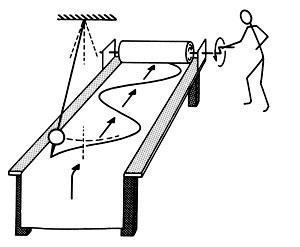
\includegraphics[width=.8 \linewidth]{bouteille_encre1.png}
        \caption{L'élongation d'un pendule en fonction du temps est une sinusoïde.}
        \label{bouteille_encre1}
    \end{minipage}
    \begin{minipage}{.5\textwidth}
        \centering
        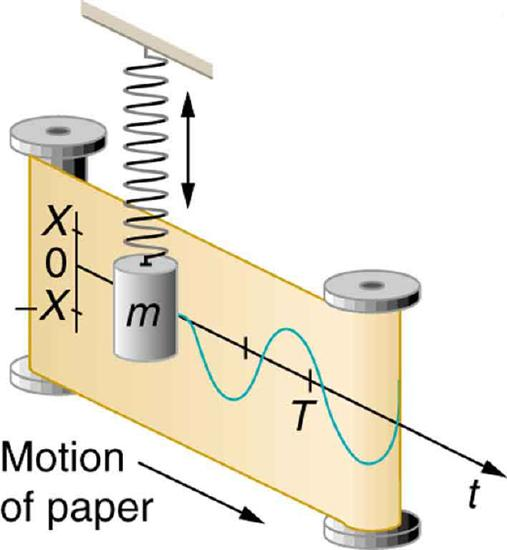
\includegraphics[width=.8 \linewidth]{bouteille_encre2.png}
        \caption{L'élongation du système masse-ressort en fonction du temps est aussi un sinusoïde.}
        \label{bouteille_encre2}
    \end{minipage}
\end{figure}

\begin{encadre}
    Un \motcle{mouvement harmonique} est un mouvement d'oscillation dont la représentation de l'élongation au cours du temps est une fonction sinusoïdale.
\end{encadre}

\newpage

\section{Exemples de mouvements simples harmoniques (MSH - SHM)}
\begin{figure}[h!]
    \centering
    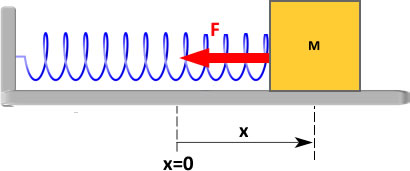
\includegraphics[width=.8 \linewidth]{bloc_ressort.png}
    \caption{Système bloc-ressort horizontal.}
    \label{bloc_ressort}
\end{figure}

\begin{figure}[h!]
    \begin{minipage}{.5\textwidth}
        \centering
        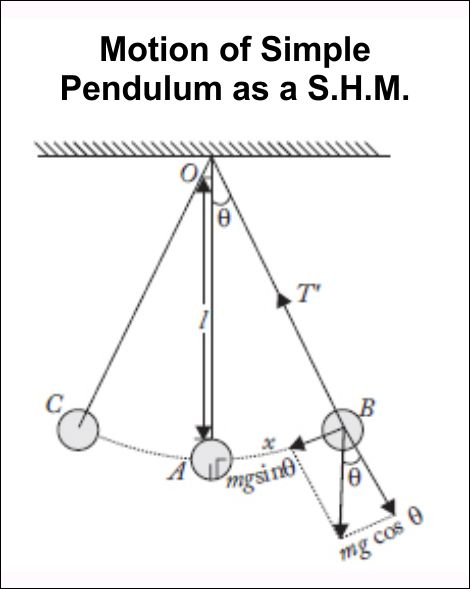
\includegraphics[width=.8 \linewidth]{pendule.png}
        \caption{Un pendule simple.}
        \label{pendule}
    \end{minipage}
    \begin{minipage}{.5\textwidth}
        \centering
        \includegraphics[width=.8 \linewidth]{bloc_ressort_2.png}
        \caption{Système bloc-ressort vertical.}
        \label{bouteille_encre3}
    \end{minipage}
\end{figure}

\newpage

\section{Le point sur le disque}
Un observateur s'intéresse à la position verticale d'un point placé sur un disque en rotation. Si le disque tourne avec une vitesse angulaire de \(\omega [rad \cdot s^{-1}]\) alors la position verticale est donnée par
\begin{equation}
    \tcboxmath[colback=LightBlue,colframe=blue]
    {x(t)=A \cdot sin(\omega t)}
\end{equation}.

\begin{figure}[h!]
    \centering
    %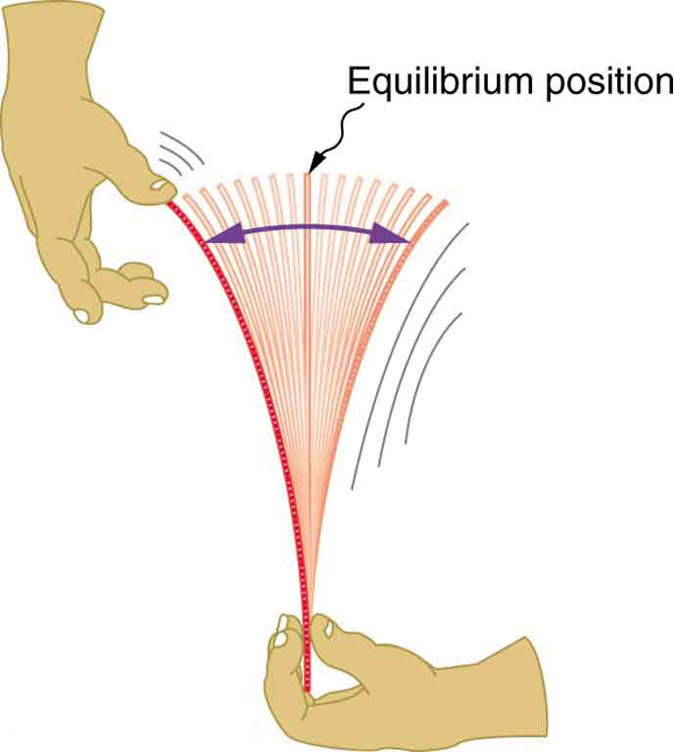
\includegraphics[width=.8 \linewidth]{latte_vibre.png}
    \includesvg[inkscapelatex=false, width=.5 \linewidth]{disque_tournant.svg}
    %\caption{}
    %\label{}
\end{figure}


Le mouvement d'un point sur un disque n'est pas l'exemple le plus évident de mouvement harmonique, mais il est facile à aborder sur le plan mathématique. Un observateur regardant le disque de côté verra le point monter et descendre comme une masse sur un ressort ou comme un pendule.
Dans le cas des mouvements harmoniques, le facteur \(\omega\) est appelé \motcle{pulsation} ou \motcle{fréquence angulaire}, il détermine le nombre de passages par la position d'équilibre que le système effectue à chaque seconde.

\newpage

\subsection{Une nouvelle vision de la vitesse et de l'accélération}
Lors des premiers cours de cinématique, la vitesse moyenne a été définie comme : \(v_{moy}=\frac{\Delta x}{\Delta t}\). Comme son nom l'indique, la vitesse moyenne est une valeur moyenne mesurée sur un intervalle de temps. Si la valeur de la vitesse moyenne est suffisante dans de nombreuses situations, il est souvent utile de connaître la valeur de la vitesse à un instant précis, c'est-à-dire la \motcle{vitesse instantanée}.
La vitesse instantanée est la valeur de la vitesse moyenne prise sur un intervalle de temps infiniment cours :\(v_{inst}= lim_{\Delta t \rightarrow 0} \frac{\Delta x}{\Delta t}\). Cela correspond à la dérivée de la position.

\begin{encadre}
    En physique, la vitesse est toujours définie comme étant la dérivée de la position par rapport au temps.
\end{encadre}

De même, l'accélération moyenne est donnée par : \(a_{moy}=\frac{\Delta v}{\Delta t}\) et l'accélération instantanée se trouve en faisant : \(a_{inst}= lim_{\Delta t \rightarrow 0} \frac{\Delta v}{\Delta t}\).

\begin{encadre}
    En physique, l'accélération est toujours définie comme étant la dérivée de la vitesse par rapport au temps.
\end{encadre}

Avec le raisonnement inverse, on comprend que la vitesse peut être trouvée en faisant l'intégrale de l'accélération et la position en faisant l'intégrale de la vitesse.

\subsection{Vérification}
L'équation horaire de la position dans le MRUA était donnée par : \(x(t)=x_0 + v_0 \cdot \Delta t + \frac{a}{2} \cdot \Delta t^2\).
La dérivée de cette fonction par rapport au temps donne : \(x'(t)=v(t)=v_0 + a \cdot \Delta t\)
Et la dérivée de celle-ci donne : \(x''(t)=v'(t)=a(t)=a\)

\begin{itemize}[label=$\rightarrow$]
    \item Détermine l'équation de la vitesse et celle de l'accélération pour le mouvement simple harmonique.
          \pointilles{5}
\end{itemize}

\newpage

\section{Le déphasage}
Que se passe-t-il si l'objet étudié n'est pas à la position \enquote{0} à l'instant \enquote{0} ?

Dans ce cas, l'écart par rapport à la position d'équilibre, appelé \motcle{constante de phase} ou \motcle{déphasage} se note \(\phi\) et l'équation de la position s'écrit :
\begin{equation}
    \tcboxmath[colback=LightBlue,colframe=blue]
    {x(t)=A \cdot sin(\omega t + \phi)}
\end{equation}

\begin{figure}[h!]
    \centering
    %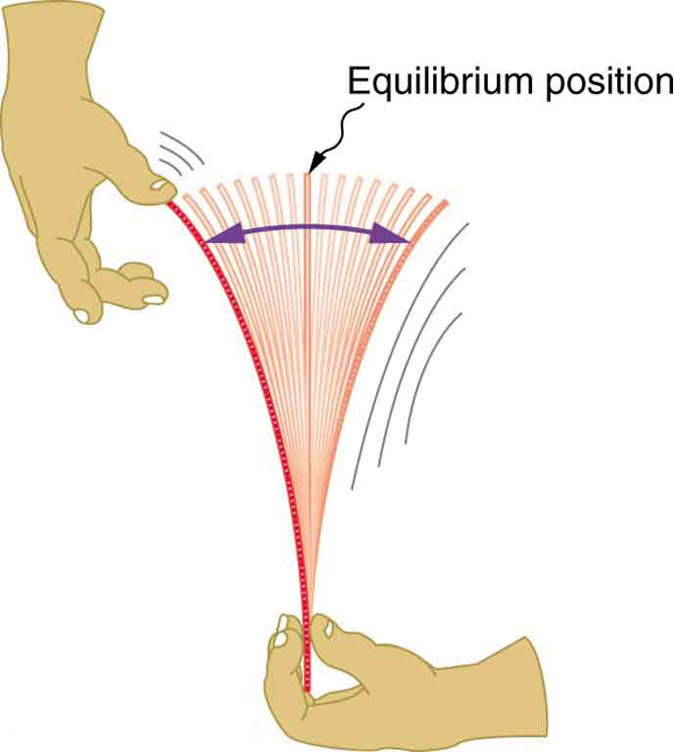
\includegraphics[width=.8 \linewidth]{latte_vibre.png}
    \includesvg[inkscapelatex=false, width=.5 \linewidth]{disque_tournant_phase.svg}
    %\caption{}
    %\label{}
\end{figure}

\newpage

\section{Exercices}
\begin{exercise}
    La position d'une particule est donnée par \(x(t)=0,03 \cdot sin(20 \pi t + \frac{\pi}{4})\)
    \begin{enumerate}[a)]
        \item Dans cette équation, identifie l'amplitude, la pulsation, le déphasage.
        \item Détermine à quel moment la position, la vitesse et l'accélération atteignent une valeur maximale positive.
    \end{enumerate}
\end{exercise}

\begin{exercise}
    Un oscillateur harmonique a pour équation de l'élongation : \(y(t)=6sin(3 \pi \cdot t + \frac{\pi}{3})\) où t est donné en secondes et y en centimètres.
    \begin{enumerate}[a)]
        \item Calcule la période du mouvement harmonique, sa fréquence et sa constante de phase.
        \item Écris l'équation de la vitesse et calcule la vitesse en \(t=3[s]\).
        \item Écris l'équation de l'accélération et calcule l'accélération en \(t=3[s]\).
    \end{enumerate}
\end{exercise}

\begin{exercise}
    Le piston d'un moteur à explosion effectue 3000 oscillations par minute.
    \begin{enumerate}[a)]
        \item Calcule sa fréquence et sa période.
        \item Si le mouvement est harmonique et que l'amplitude vaut \(5cm\), calcule la vitesse maximale du piston.
        \item Calcule son accélération maximale.
        \item Si la masse du piston est de \(100g\), calcule la force maximale s'exerçant sur lui.
    \end{enumerate}
\end{exercise}

Exercices supplémentaires :\\
\qrcode{https://www.vf-bxl-moodle.be/mod/quiz/view.php?id=1370}


\newpage

\section{Caractéristiques du MSH}
Nous allons mettre en évidence les conditions dans lesquelles un mouvement simple harmonique apparaît.
L'équation horaire de l'accélération montrait que \(a(t)=- \omega ^2 \cdot  x(t)\). Si on souhaite connaître la façon dont la force qui crée le SHM varie, on obtient : \(F(t)=- m \cdot \omega ^2 \cdot x(t)\). Les paramètres \(m\) et \(\omega\) sont constants, donc le produit \(m \cdot \omega\) aussi une constante. Il est donc permis d'écrire : \(F(t)=- k \cdot x(t)\).

Cette dernière équation montre que dans un MSH :
\begin{enumerate}[(a)]
    \item la force qui crée le mouvement est proportionnelle à l'élongation ;
    \item cette force est opposée à l'élongation, c'est une \motcle{force de rappel}.
\end{enumerate}


Toute situation dans laquelle une telle force est observée va engendrer un MSH. De la même manière, une situation dans laquelle il existe une force constante centripète crée un MCU ou une situation dans laquelle il existe une force constante dans le sens du déplacement crée un MRUA.


\begin{figure}[h!]
    \centering
    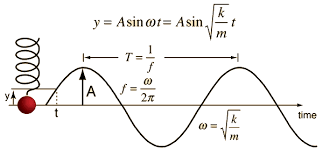
\includegraphics[width=.5 \linewidth]{shm.png}
    %\includesvg[inkscapelatex=false, width=.5 \linewidth]{tir_oblique.svg}
    \caption{Un mouvement simple harmonique}
    \label{shm}
\end{figure}

\chapter{Le système masse-ressort}
Le système masse-ressort constitue en une masse suspendue à un ressort. Il peut aussi s'agir d'une masse posée sur une surface plane et reliée à un ressort. Il n'y a pas de frottements entre la masse et la surface plane.

\begin{figure}[ht!]
    \begin{minipage}{.5\textwidth}
        \centering
        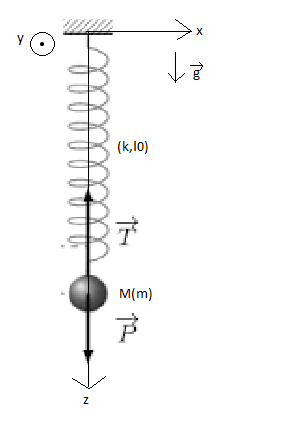
\includegraphics[width=.8 \linewidth]{masse_ressort_I.png}
        \caption{Système masse ressort.}
        \label{masse_ressort_I}
    \end{minipage}
    \begin{minipage}{.5\textwidth}
        \centering
        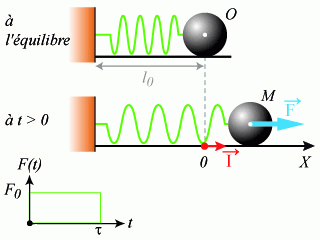
\includegraphics[width=.8 \linewidth]{bloc_ressort_I.png}
        \caption{Système bloc-ressort horizontal.}
        \label{bloc_ressort_I}
    \end{minipage}
\end{figure}

\newpage

Si la masse est déplacée vers la gauche par rapport à sa position d'équilibre, le ressort exerce une force opposée  et proportionnelle au déplacement. Une telle situation correspond aux conditions du MSH.
Dans le système masse ressort, la constante de proportionnalité liant l'élongation à la force de rappel est la constante de raideur du ressort. Puisque \(k=m \cdot \omega ^2\) alors :

\begin{equation}
    \tcboxmath[colback=LightBlue,colframe=blue]
    {\omega = \sqrt{\frac{k}{m}}}
\end{equation}


Si on se rappelle que \(\omega=2 \cdot \pi \cdot f\), on déduit que :

\begin{equation}
    \tcboxmath[colback=LightBlue,colframe=blue]
    {f=\frac{1}{2\pi} \cdot \sqrt{\frac{k}{m}}}
\end{equation}

\newpage

\section{Exercices}
\begin{exercise}
    Un oscillateur effectue 20 allers-retours en \(5,64 secondes\). L'objet en oscillation a une masse de \(145g\). Calcule la constante de raideur du ressort.
\end{exercise}
\begin{solution}
    \(k=71,983 N/m\)
\end{solution}

\begin{exercise}
    Il faut une force de 0,064N pour éloigner de 4cm un ressort de sa position d'équilibre. On y attache un objet dont la masse est de 200g et on laisse osciller le tout librement. Calcule la période et la fréquence du mouvement.
\end{exercise}
\begin{solution}
    \(f=0,45 Hz ; T=2,221 s\)
\end{solution}

\begin{exercise}
    Un objet d'une masse de 500[g] est attaché à un ressort. Le graphique ci-dessous représente son élongation au cours du temps.
    \begin{enumerate}[a)]
        \item Calcule la constante de raideur du ressort.
        \item Calcule l'intensité de la force résultante agissant sur l'objet lorsque l'élongation est maximale.
    \end{enumerate}
    \begin{figure}[ht!]
        \centering
        \begin{tikzpicture}[scale=0.75]
            \tikzset{>=latex}
            \tkzInit[xmin=0,xmax=1,ymin=-10,ymax=10,xstep=0.1,ystep=2]
            \tkzGrid
            \tkzDrawX[label={$t [s]$},below left=25pt]
            \tkzDrawY[label={$Y [mm]$},right=5pt]
            \tkzAxeXY[label={}] %This macro combines the four macros: \tkzDrawX\tkzDrawY \tkzLabelX\tkzLabelYnode font=\tiny]
            \tkzFct[domain=0:1,red]{8*sin(0.5*pi*x)}
        \end{tikzpicture}
    \end{figure}
\end{exercise}
\begin{solution}
    \(k=123,37 N/m\)
\end{solution}

\begin{exercise}
    \begin{minipage}[t]{0.4\textwidth}
        \qrcode{https://www.vf-bxl-moodle.be/mod/quiz/view.php?id=1369}
    \end{minipage}
\end{exercise}

\chapter{Le pendule}
Un pendule simple est un système idéalisé constitué d'une masse ponctuelle suspendue à l'extrémité d'un fil inélastique de masse négligeable.

L'étude du pendule offre un bel exemple de la validité des lois en physique : le plus souvent, celles-ci ne sont vraies que dans certaines conditions et il en existe des formulations plus générales, mais plus complexes.

Un exemple célèbre est celui des phénomènes relativistes comme l'augmentation de la masse inertielle en fonction de la vitesse : \(m=\frac{m_0}{\sqrt{1-\frac{v^2}{c^2}}}\). La masse des corps est généralement considérée comme constante, mais il s'agit d'une simplification valable pour des vitesses petites par rapport à celle de la lumière.

Considérer que le mouvement d'un pendule est un MSH est une simplification qui n'est valable que pour les petits angles, cette limitation est connue comme \enquote{\motcle{l'approximation des petits angles}}.

\newpage

\section{Approximation des petits angles}
Les graphiques ci-dessous présentent les fonctions \textcolor{OliveGreen}{\(f(x)=x\)} et \textcolor{red}{\(g(x)=sin(x)\)}.

\begin{figure}[ht!]
    \begin{minipage}{.5\textwidth}
        \centering
        \begin{tikzpicture}[scale=0.55]
            \tikzset{>=latex}
            \tikzstyle{every node}=[font=\tiny]
            \tkzInit[xmin=-2,xmax=3,ymin=-2,ymax=3,xstep=0.5,ystep=0.5]
            \tkzGrid
            \tkzDrawX[label={$X$}]
            \tkzDrawY[label={$Y$}]
            %\tkzAxeXY
            \tkzAxeXY[label={}] %This macro combines the four macros: \tkzDrawX\tkzDrawY \tkzLabelX\tkzLabelYnode font=\tiny]
            \tkzFct[domain=-2:3,color=red]{sin(\x)}
            \tkzFct[domain=-2:3,color=OliveGreen]{\x}
        \end{tikzpicture}
        %\includegraphics[width=.8 \linewidth]{fonctions_x_sin_x_I.png}
        \caption{Les fonctions \(f(x)=x\) et \(g(x)=sin(x)\)}
        \label{fonctions_x_sin_x_I}
    \end{minipage}
    \begin{minipage}{.5\textwidth}
        \centering
        \begin{tikzpicture}[scale=0.55]
            \tikzset{>=latex}
            \tikzstyle{every node}=[font=\tiny]
            \tkzInit[xmin=-0.05,xmax=0.45,ymin=-0.05,ymax=0.45,xstep=0.05,ystep=0.05]
            \tkzGrid
            \tkzDrawX[label={$X$}]
            \tkzDrawY[label={$Y$}]
            %\tkzAxeXY
            \tkzAxeXY[label={}] %This macro combines the four macros: \tkzDrawX\tkzDrawY \tkzLabelX\tkzLabelYnode font=\tiny]
            \tkzFct[domain=0:.5,color=red]{sin(\x)}
            \tkzFct[domain=0:.5,color=OliveGreen]{\x}
        \end{tikzpicture}
        \caption{Les fonctions \(f(x)=x\) et \(g(x)=sin(x)\)}
        \label{fonctions_x_sin_x_II}
    \end{minipage}
\end{figure}

On remarque que lorsque x est petit, l'écart entre \(f(x)\) et \(g(x)\) est négligeable, il est donc permis de considérer que si x est petit alors \(sin(x)=x\). En pratique, cette approximation est utilisée pour des angles inférieurs à 0,1 rad, c'est-à-dire \(6^\circ\).

\newpage

\section{Équation horaire du pendule simple}
Pour étudier le pendule simple, nous utiliserons un référentiel dont les deux axes sont toujours perpendiculaires et tangents à la trajectoire.
Dans ce système d'axes, les forces qui s'exercent sur la masse \enquote{m} sont son poids, \(\vec{F_g}\), et la traction du fil, \(\vec{T}\). Le poids peut être décomposé en \(\vec{F_{gX}}\), tangent à la trajectoire et \(\vec{F_{gY}}\) perpendiculaire à celle-ci.
On peut donc écrire que :
\begin{itemize}
    \item \(F_{gX}=m \cdot g  \cdot sin(\theta)\)
    \item \(F_{gY}=m \cdot g  \cdot cos(\theta)\)
\end{itemize}



La force qui rappelle la masse vers sa position d'équilibre est \(\vec{F_{gX}}\), donc :
\begin{align}
    F(t)=F_{gX}=m \cdot g \cdot sin(\theta)
\end{align}
Dans cette équation, si \(\theta <<<\), alors \(sin(\theta)=\theta\) et donc :
\begin{align}
    F(t)=m \cdot g \cdot \theta
\end{align}


\begin{figure}[ht!]
    \centering
    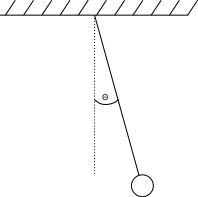
\includegraphics[width=.5 \linewidth]{demo_pendule.png}
    \caption{Les forces agissant sur un pendule simple}
    \label{demo_pendule_I}
\end{figure}

\newpage

Pour pouvoir aller plus loin, il faut exprimer l'écartement par rapport à la position d'équilibre en fonction de l'élongation et non en fonction de \(\theta\).
Pour cela, nous allons utiliser une autre approximation.
Si \(\theta\) est petit, alors l'élongation \enquote{y} peut être approximée par la longueur de l'arc OM (voir \cref{fig:demo_pendule_II} \cpageref{fig:demo_pendule_II}).
Dès lors :
\begin{equation}
    y=L \cdot \theta \ \rightarrow \ \theta=\frac{y}{L}
\end{equation}
L'équation de la force engendrant le MSH devient donc :
\begin{align}
    F(t)=m \cdot g \cdot \frac{y}{L} \rightarrow \\
    F(t)=\frac{m \cdot g}{L} \cdot y
\end{align}

On retrouve alors la structure d'une équation du MSH : une force proportionnelle à une élongation.
Dans cette équation, la constante du MSH vaut :
\begin{equation}
    \label{eqn:k_msh_I}
    k_{MSH}=\frac{m \cdot g}{L}
\end{equation}
Étant donné que l'impulsion vaut :
\begin{equation}
    \label{eqn:k_msh_II}
    k_{MSH}=m \cdot \omega^2
\end{equation}
On peut égaler ces deux équations (\ref{eqn:k_msh_I} et \ref{eqn:k_msh_II}) pour obtenir :
\begin{equation}
    \frac{m \cdot g}{L} = m \cdot \omega^2
\end{equation}

On voit que la masse se simplifie et qu'on obtient :
\begin{align}
    \omega^2=\frac{g}{L}
\end{align}

Conclusion : l'impulsion d'un pendule ne dépend pas de la masse, mais uniquement de la longueur du pendule.
\begin{equation}
    \tcboxmath[colback=LightBlue,colframe=blue]{\omega = \sqrt{\frac{g}{L}}}
\end{equation}


\begin{figure}[ht!]
    \centering
    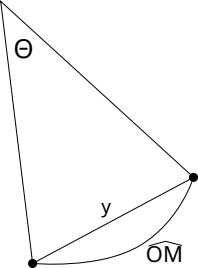
\includegraphics[width=.3 \linewidth]{demo_pendule_II.png}
    \caption{Approximation de l'élongation par l'arc de cercle.}
    \label{fig:demo_pendule_II}
\end{figure}

\newpage

\section{Exercices}
\begin{exercise}
    Un pendule effectue 30 allers-retours en 10 secondes.
    \begin{enumerate}[a)]
        \item Quelle est la longueur du pendule ?
        \item Quelle devrait être la longueur pour diviser la fréquence par 2 ?
    \end{enumerate}
\end{exercise}

\begin{exercise}
    Une balançoire est attachée à la branche d'un arbre, mais celle-ci est inclinée et forme un angle de \(20^{\circ}\). La distance entre les deux points d'attache est de 70cm et la plus petite corde de la balançoire mesure \(3[m]\).
    \begin{enumerate}[a)]
        \item Comment la balançoire va-t-elle se comporter ?
        \item La balançoire est écartée de 1[m] puis est lachée. Où se trouvent les deux points d'attache 10[s] après le premier passage par la position d'équilibre ?
    \end{enumerate}
\end{exercise}

\begin{exercise}
    Un pendule d'une longueur de 50[cm] est écarté de 4[cm] par rapport à sa position d'équlibre.
    \begin{enumerate}[a)]
        \item Quelle est sa vitesse après 10[s] ?
        \item Quelle est sa fréquence ?
    \end{enumerate}
\end{exercise}
\begin{solution}
    \begin{itemize}
        \item \(v(10)=0,1686 [m/s]\)
        \item \(f=0,70497[Hz]\)
    \end{itemize}
\end{solution}


\begin{minipage}{.5\textwidth}
    \begin{exercise}
        \qrcode{https://www.vf-bxl-moodle.be/mod/quiz/view.php?id=1441}
    \end{exercise}
\end{minipage}
\begin{minipage}{.5\textwidth}
    \begin{exercise}
        \qrcode{https://www.vf-bxl-moodle.be/mod/quiz/view.php?id=1437}
    \end{exercise}
\end{minipage}




\chapter{Oscillateurs couplés et résonance}
Lorsqu'un système entre en vibration, il oscille à sa fréquence naturelle. Cette fréquence dépend des propriétés du système : constante de raideur et masse pour masse-ressort, longueur pour les pendules ou un ensemble de propriétés plus ou moins complexes pour d'autres systèmes.

Toutefois, pour amorcer l'oscillation d'un système, une force a dû s'appliquer dessus et si on souhaite maintenir les oscillations, la force doit s'exercer périodiquement sur celui-ci. Si la force qui s'applique sur l'oscillateur s'exerce avec une fréquence différente de la fréquence naturelle, l'oscillateur va adopter celle-ci. On parle alors d'\motcle{oscillations forcées}.
Si, au contraire, la fréquence avec laquelle on excite oscillateur correspond à sa fréquence naturelle, celui-ci va entrer en \motcle{résonance} et l'amplitude du mouvement va devenir de plus en plus grande.

\begin{figure}[ht!]
    \centering
    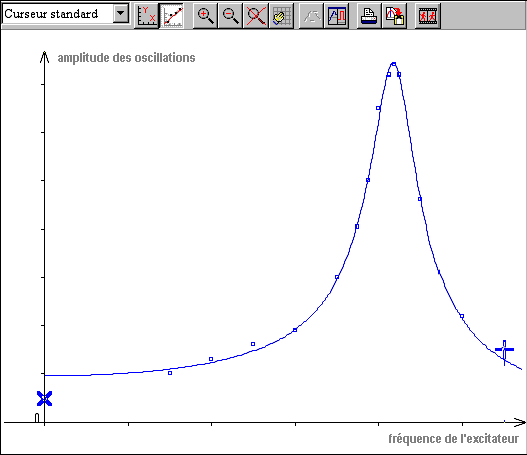
\includegraphics[width=.5 \linewidth]{resonnance.png}
    \caption{Amplitude d'un oscillateur en fonction de la fréquence d'excitation.}
    \label{resonnanceI}
\end{figure}

\begin{encadre}
    Lorsque deux oscillateurs de même fréquence sont reliés entre eux, le premier communique progressivement son énergie au deuxième, ils sont en \motcle{résonance}.
\end{encadre}

\newpage

\section{Oscillateurs couplés}
Lorsque deux pendules de même fréquence sont couplés, ils entrent en résonance et toute l'énergie du premier va être communiquée au deuxième qui la communique à son tour au premier et ainsi de suite. Ce transfert est d'autant plus efficace si leurs fréquences naturelles sont proches et que le couplage est rigide.

\begin{figure}[ht!]
    \centering
    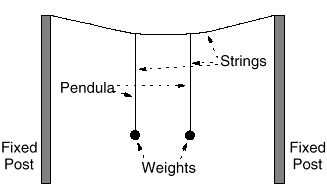
\includegraphics[width=.5 \linewidth]{resonnance_II.png}
    \caption{Deux oscillateurs de même fréquence propre rentrent en résonance lorsqu'ils sont couplés.}
    \label{resonnanceII}
\end{figure}

Si un grand nombre d'oscillateurs sont couplés de manière à former une chaîne, la perturbation du premier va progressivement se transmettre le long de cette chaîne. Il en résulte une propagation d'énergie sous forme d'énergie cinétique et potentielle sans que les oscillateurs ne se déplacent le long de la chaîne, c'est une \motcle{onde}.

\begin{figure}[ht!]
    \centering
    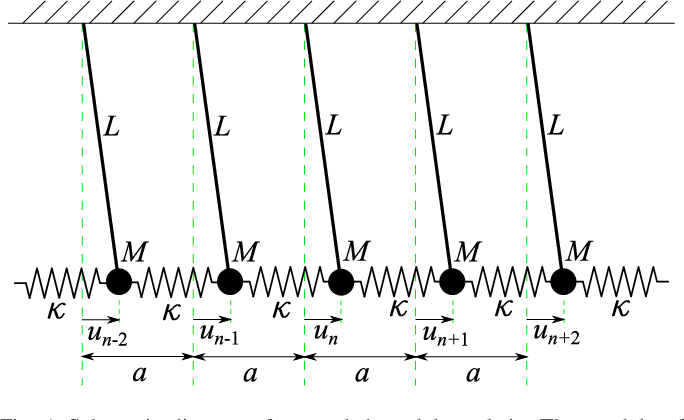
\includegraphics[width=.5 \linewidth]{resonnance_III.png}
    \caption{Cinq oscillateurs couplés.}
    \label{resonnanceIII}
\end{figure}


\begin{encadre}
    Une \motcle{onde mécanique} est un transfert de proche en proche d'un signal à travers un milieu ; ce signal consiste en la modification d'une propriété physique du milieu : position de la matière, pression, ...
    La propagation d'une onde s'accompagne d'un transfert d'énergie, mais pas d'un transfert de matière.
\end{encadre}

\chapter{Les ondes mécaniques}
Lorsqu'un caillou tombe dans l'eau, l'eau qui se trouve au point d'impact va osciller et cette oscillation va se transmettre à toutes les molécules environnantes et il se forme une onde circulaire. Un bouchon qui flotte à proximité du point d'impact va monter et descendre au passage de la perturbation, mais il ne va pas avancer.

\begin{figure}[ht!]
    \centering
    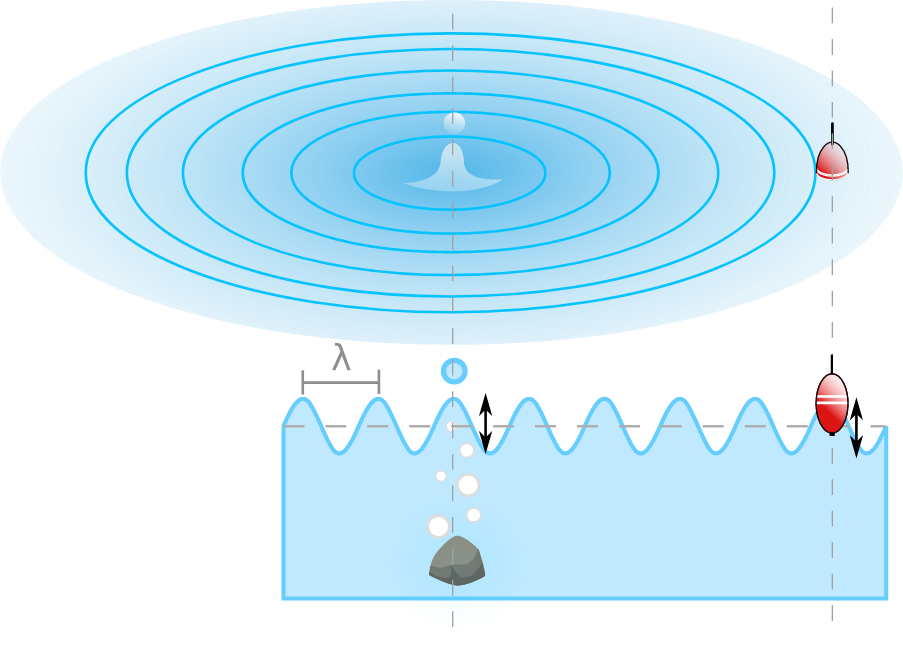
\includegraphics[width=.5 \linewidth]{onde_mecanique.png}
    \caption{Le bouchon à la surface de l'eau.}
    \label{onde_mecanique}
\end{figure}

\newpage

\section{Classification des ondes}
Il existe de nombreux critères sur base desquels classer les ondes mécaniques : milieu de propagation, vitesse, direction de la perturbation. Si on se réfère à la direction de propagation, deux grandes catégories existent :
\begin{itemize}[label=\textbullet]
    \item \motcle{Ondes transversales}
          \pointilles{3}
    \item \motcle{Ondes longitudinales}
          \pointilles{3}
\end{itemize}

\begin{figure}[ht!]
    \centering
    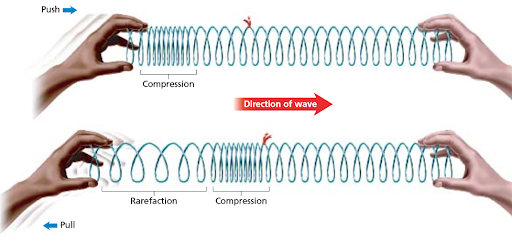
\includegraphics[width=.75 \linewidth]{ondes_longitudinales.png}
    \caption{Un exemple d'onde longitudinale}
    \label{onde_longitudinale}
\end{figure}

\begin{figure}[ht!]
    \centering
    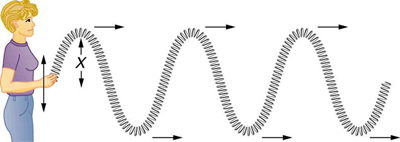
\includegraphics[width=.75 \linewidth]{ondes_transversales.png}
    \caption{Un exemple d'onde transversale}
    \label{onde_transversale}
\end{figure}

\newpage

\section{Vitesse d'une onde}
La vitesse d'une onde mécanique dépend uniquement des propriétés du milieu dans lequel elle circule. Cela implique que cette vitesse ne dépend pas de l'amplitude. En règle générale, plus le milieu est dense, plus la vitesse est élevée.
Si le milieu est homogène, la vitesse de l'onde est constante et les lois du MRU peuvent être utilisées pour connaître les caractéristiques de la perturbation : position, vitesse, durée.

\begin{center}
    \begin{tabularx}{.8 \textwidth}{m{.4 \textwidth} X}
        \hline
        \uppercase{Phénomène} & \uppercase{Vitesse}[m/s]        \\
        \hline
        Son dans l'air        & 340                             \\
        \hline
        Son dans l'eau        & 1500                            \\
        \hline
        Onde sismique         & 4060                            \\
        \hline
        Lumière               & 300 000 000 (\(3 \times 10^8\)) \\
        \hline
    \end{tabularx}
\end{center}


\subsection{Applications}
\begin{enumerate}[a)]
    \item En utilisant la formule de la vitesse moyenne (\(v_{moy}=\frac{\Delta x}{\Delta t}\)) calcule le temps pris par la lumière d'un éclair pour parcourir une distance équivalente à la circonférence de la Terre (\(r_{Terre} = 6400 [ km]\)).
    \item Détermine la distance à laquelle se trouve un orage s'il s'écoule 6 secondes entre la perception de l'éclair et celle du tonnerre sachant que ces deux phénomènes sont simultanés.
\end{enumerate}

\newpage

\section{Onde unique et onde entretenue}
\label{Onde unique et onde entretenue}
Une onde est une perturbation qui se propage. Cette perturbation peut être unique ou se répéter dans le temps. Dans ce cas, l'onde devient une \motcle{onde continue} ou onde entretenue.

\begin{figure}[ht!]
    \centering
    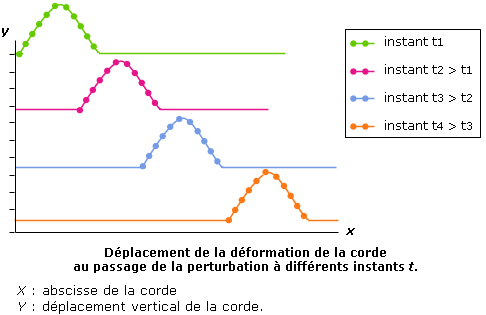
\includegraphics[width=.75 \linewidth]{onde_unique.png}
    \caption{Une onde provoquée par une impulsion unique.}
    \label{onde_unique}
\end{figure}

\newpage

\section{La longueur d'onde}
Pour une onde continue, il existe un nouveau paramètre permettant de les caractériser : leur \motcle{longueur d'onde}.
\begin{itemize}[label=\textbullet]
    \item \motcle{Longueur d'onde}
          \pointilles{3}
\end{itemize}

\begin{figure}[ht!]
    \centering
    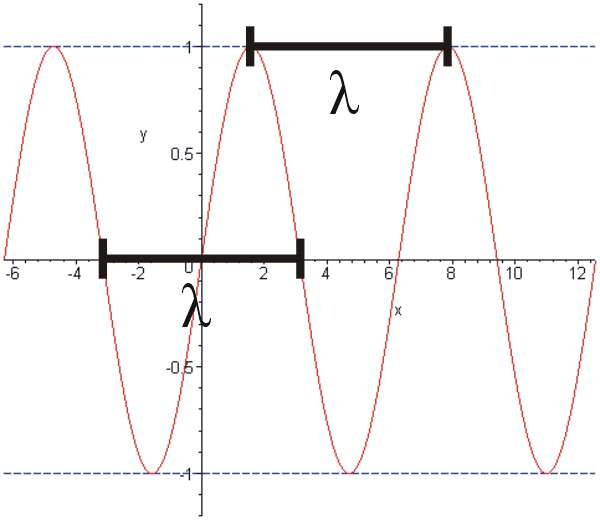
\includegraphics[width=.75 \linewidth]{longueur_onde.png}
    \caption{La longueur d'onde}
    \label{longueur_onde}
\end{figure}

\newpage

\section{Relation fréquence, vitesse, longueur d'onde}
Le schéma ci-dessous représente une onde continue. À partir de ce schéma, établi le lien entre la longueur d'onde, la vitesse et la fréquence de l'onde.
\begin{itemize}[label=\textbullet]
    \item
          \pointilles{2}
\end{itemize}
\begin{figure}[ht!]
    \centering
    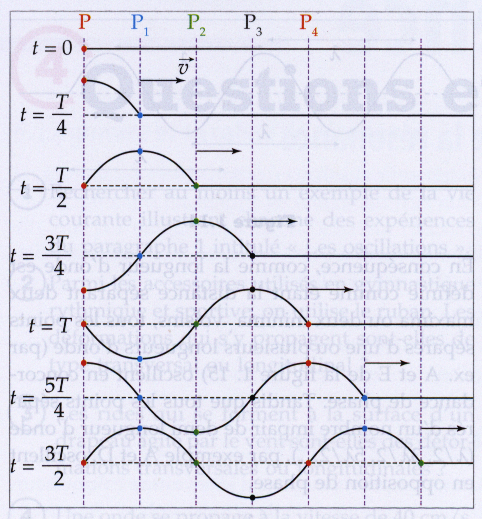
\includegraphics[width=.75 \linewidth]{relation_vitesse_frequence.png}
    \caption{Une onde continue}
    \label{relation_vitesse_frequence}
\end{figure}

Nous avons vu que la vitesse d'une onde dépend des caractéristiques du milieu de propagation. Quel serait, selon toi, l'effet d'une augmentation de la fréquence sur les caractéristiques de l'onde ?

\begin{itemize}[label=\textbullet]
    \item
          \pointilles{2}
\end{itemize}

\section{Élongation d'un point au cours du temps}
Lorsqu'il est atteint par l'onde, chaque point du milieu de propagation se comporte comme un oscillateur harmonique. Nous allons établir l'équation donnant l'élongation en fonction du temps pour un point \(P\) se trouvant à une distance \(x\) de la source \(S\).

\begin{figure}[ht!]
    \centering
    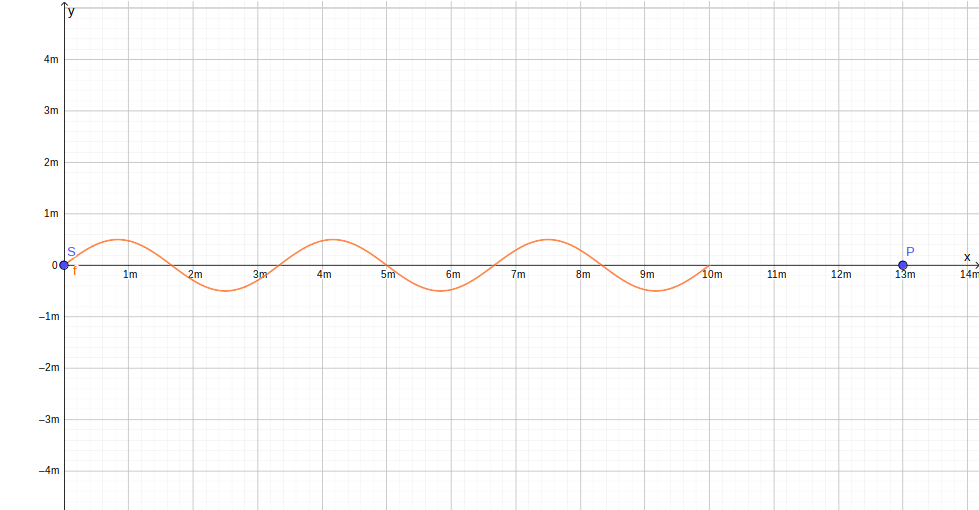
\includegraphics[width=.75 \linewidth]{equation_elongation.png}
    \caption{Élongation en fonction de la distance pour une onde continue.}
    \label{equation_elongation}
\end{figure}

La source se comporte comme un oscillateur harmonique, son élongation est donnée par  \(y_S (t)=A \cdot sin(\omega \cdot t)\).
Si le milieu est homogène, l'élongation du point sera la même que celle de la source, mais avec un décalage dans le temps. On peut donc écrire :
\begin{equation}
    y_P (t + \Delta t)   = y_S (t)
\end{equation}
où \(\Delta t\) est le temps pris par l'onde pour atteindre le point \(P\).
On peut écrire différemment l'équation ci-dessous :
\begin{equation}
    y_P (t)   = y_S (t - \Delta t)
\end{equation}
Le point P se comporte à l'instant \(t\) comme la source se comportait il y a \(\Delta t\) secondes.
On peut donc dire que :
\begin{align}
    y_P (t) & = A \cdot sin (\omega \cdot(t-\Delta t))             \\
    y_P (t) & = A \cdot sin (\omega \cdot t-\omega \cdot \Delta t)
    \label{eqn:position1}
\end{align}
Or, nous savons que \(\Delta t =\frac{x}{v}\). L'équation \ref{eqn:position1} devient alors :
\begin{align}
    y_P (t) & = A \cdot sin (\omega \cdot t-\omega \cdot \frac{x}{v})
    \label{eqn:position2}
\end{align}

Nous savons aussi que \(\omega = 2 \pi \cdot f\), l'équation \ref{eqn:position2} peut donc s'écrire :
\begin{align}
    y_P (t) & = A \cdot sin (\omega \cdot t-2 \pi f \cdot \frac{x}{\lambda \cdot f})
    \label{eqn:position3}
\end{align}

Finalement, on simplifie l'équation \ref{eqn:position3} qui devient :
\begin{equation}
    \tcboxmath[colback=LightBlue,colframe=blue]{y_P (t)= A \cdot sin (\omega \cdot t- \frac{2 \pi  \cdot x}{\lambda})}
\end{equation}

\newpage

\section{La double périodicité des ondes}
\subsection{Périodicité dans le temps}
Dans l'équation de l'élongation en fonction de la position et du temps, si on considère un point fixe, alors le terme \(\frac{2 \pi \cdot x}{\lambda}\) est une constante et l'équation peut s'écrire : \(y_P (t) = A \cdot sin (\omega \cdot t- cst)\). Cela correspond exactement à l'équation d'un mouvement simple harmonique avec une constante de phase égale à : \(\phi = \frac{2 \pi \cdot x}{\lambda}\).

\begin{encadre}
    Chaque point oscille avec la même amplitude et la même fréquence que la source, mais avec un déphasage d'autant plus grand que ce point est éloigné de la source.
\end{encadre}

\subsection{Périodicité dans l'espace}
Si on s'intéresse à l'aspect de l'onde à un instant donné, une photographie de l'onde présentant l'élongation de tous les points alors l'équation de l'onde devient : \(y (x) = A \cdot sin (cst - \frac{2 \pi  \cdot x}{\lambda})\). Cette équation montre qu'à chaque instant l'ensemble des points en oscillation forment une sinusoïde.

\begin{encadre}
    Les ondes continues présentent une double périodicité :
    \begin{itemize}
        \item périodicité dans le temps pour chaque point ;
        \item périodicité dans l'espace pour l'ensemble des points à chaque instant.
    \end{itemize}
\end{encadre}

\newpage

\section{Opposition et concordance de phase}
Sur une onde continue, certains points oscillent de la même manière : ils sont toujours à leur amplitude minimale, maximale ou nulle en même temps. Deux points qui oscillent avec la même élongation sont dits en \motcle{concordance de phase}. Tandis que deux points qui ont toujours une élongation opposée sont dits en \motcle{opposition de phase}.
\begin{itemize}[label=\textbullet]
    \item À quelle condition deux points sont-ils en concordance de phase ?
          \pointilles{2}
    \item À quelle condition deux points sont-ils en opposition de phase ?
          \pointilles{2}
\end{itemize}

\begin{figure}[ht!]
    \centering
    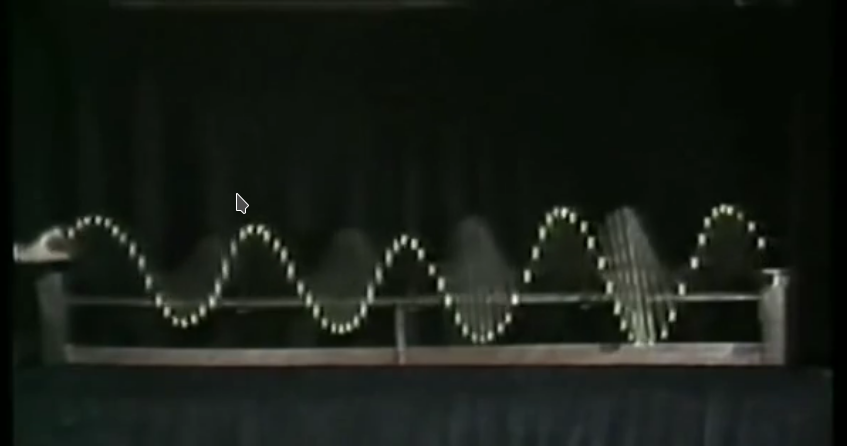
\includegraphics[width=.75 \linewidth]{onde_shive.png}
    \caption{Une onde sur la machine de Shive.}
    \label{onde_shive}
\end{figure}

\chapter{Caractéristiques des ondes mécaniques}
\section{Principe de superposition des ondes}
Quand deux ondes ou plus passent en même temps par une même région de l'espace, on observe que le déplacement réel est la somme vectorielle des déplacements causés par chaque onde individuelle.
C'est le \motcle{principe de superposition des ondes}.
Les illustrations ci-dessous présentent respectivement deux ondes puis la superposition de celles-ci.
\begin{figure}[ht]
    \begin{tikzpicture}
        \definecolor{olivegreen}{RGB} {0,125,15}
        \tikzset{>=latex}
        \tkzInit[xmin=-4,xmax=8,ymin=-1,ymax=1.5,xstep=1,ystep=1]
        \tkzDrawX[label={$X [m]$},below left=25pt]
        \tkzDrawY[label={$Y [m]$},right=5pt]
        \tkzAxeXY[label={}] %This macro combines the four macros: \tkzDrawX\tkzDrawY \tkzLabelX\tkzLabelYnode font=\tiny]
        \tkzFct[domain=-4:8,red]{sin(pi*x)}
    \end{tikzpicture}
    %\label{Une onde dont l'équation de l'élongation est donnée par \(y(t)=sin( \pi \cdot t) \)}
    \caption{Une onde dont l'équation de l'élongation est donnée par \(y(t)=sin( \pi \cdot t) \)}
\end{figure}

\begin{figure}[ht]
    \begin{tikzpicture}
        \definecolor{olivegreen}{RGB} {0,125,15}
        \tikzset{>=latex}
        \tkzInit[xmin=-4,xmax=8,ymin=-1,ymax=1.5,xstep=1,ystep=1]
        \tkzDrawX[label={$X [m]$},below left=25pt]
        \tkzDrawY[label={$Y [m]$},right=5pt]
        \tkzAxeXY[label={}] %This macro combines the four macros: \tkzDrawX\tkzDrawY \tkzLabelX\tkzLabelYnode font=\tiny]
        \tkzFct[domain=-4:8,red]{sin(2*pi*x)}
    \end{tikzpicture}
    %\label{Une onde dont l'équation de l'élongation est donnée par \(y(t)=sin( \pi \cdot t) \)}
    \caption{Une onde dont l'équation de l'élongation est donnée par \(y(t)=sin(2 \cdot \pi \cdot t) \)}
\end{figure}

\begin{figure}[ht]
    \begin{tikzpicture}
        \definecolor{olivegreen}{RGB} {0,125,15}
        \tikzset{>=latex}
        \tkzInit[xmin=-4,xmax=8,ymin=-2,ymax=2.5,xstep=1,ystep=1]
        \tkzDrawX[label={$X [m]$},below left=25pt]
        \tkzDrawY[label={$Y [m]$},right=5pt]
        \tkzAxeXY[label={}] %This macro combines the four macros: \tkzDrawX\tkzDrawY \tkzLabelX\tkzLabelYnode font=\tiny]
        \tkzFct[domain=-4:8,red]{sin(2*pi*x)+sin(pi*x)}
    \end{tikzpicture}
    %\label{Une onde dont l'équation de l'élongation est donnée par \(y(t)=sin( \pi \cdot t) \)}
    \caption{Une onde dont l'équation de l'élongation est donnée par \(y(t)=sin( \pi \cdot t)+sin(2 \cdot \pi \cdot t) \)}
\end{figure}

\newpage

Ce principe de superposition n'est valable que lorsque les élongations ne sont pas trop importantes et lorsque la force de rappel est proportionnelle au déplacement.
L'onde résultante n'est pas une onde sinusoïdale simple, on parle dans ce cas d'\motcle{onde composite}. On peut démontrer que toute onde composite peut être considérée comme étant composée de plusieurs ondes sinusoïdales simples de fréquence et amplitudes différentes. Ce concept a été introduit par Joseph Fourier en 1822. L'ensemble des ondes qui se combinent pour former une onde composite est appelé \motcle{série de Fourier}.
Les ondes simples qui se combinent pour former l'onde composite sont appelées \motcle{harmoniques} de l'onde. L'harmonique de plus petite fréquence, et dont les autres ne sont qu'un multiple, est appelée \motcle{harmonique fondamentale}.
Les séries de Fourier se rencontrent dans la décomposition de signaux périodiques, dans l'étude des courants électriques, des ondes cérébrales, dans la synthèse sonore, le traitement d'images, etc.
\newpage

\begin{figure}[ht]
    \centering
    \includegraphics[width=.4\linewidth]{serie_fourier.png}
    \caption{Les quatre premières sommes partielles de la série de Fourier pour un signal carré.}
\end{figure}

\newpage

\section{Réflexion des ondes}
Lorsqu'une onde rencontre un obstacle ou qu'elle arrive à la fin du milieu dans lequel elle se propage, elle est au moins partiellement réfléchie.
Une onde ne se réfléchi pas de la même manière selon que l'extrémité du milieu soit fixe ou mobile.
\begin{figure}[ht]
    \begin{minipage}{.5\textwidth}
        \centering
        \includegraphics[width=.8 \linewidth]{reflexion_fixee.png}
        \caption{Réflexion d'une onde dont l'extrémité est fixée.}
    \end{minipage}
    \begin{minipage}{.5\textwidth}
        \centering
        \includegraphics[width=.8 \linewidth]{reflexion_libre.png}
        \caption{Réflexion d'une onde dont l'extrémité est libre.}
    \end{minipage}
\end{figure}
On observe que lorsque l'extrémité est fixée, l'onde réfléchie est inversée ce qui n'est pas le cas lorsque l'extrémité est libre. Cela s'explique, car lorsque l'onde atteint l'extrémité fixée, elle exerce une force vers le haut sur le support qui, en retour, exerce une force réciproque vers le bas sur le support de l'onde (la corde ou autre chose).
Dans le cas d'une onde à deux ou trois dimensions, comme les vagues sur l'eau, il importe de considérer le \motcle{front} de l'onde, c'est-à-dire toute la largeur de la crête de l'onde, la ligne formée par tous les points oscillant en phase.
On appelle \motcle{rayon}, toute ligne de même direction que le déplacement de l'onde et perpendiculaire au front de celle-ci.

\newpage

\subsection{Loi de la reflexion}
Lorsqu'une onde est réfléchie sur une surface, l'angle d'incidence est égal à l'angle de réflexion. Ces deux angles, sont ceux entre le rayon de l'onde et la perpendiculaire à la surface de réflexion.
\begin{encadre}
    \(\theta_i = \theta_r\)
\end{encadre}

\begin{tikzpicture}[line cap=round,line join=round,>=triangle 45,x=1cm,y=1cm,use optics]
    \fill[line width=0pt,color=Brown,fill=Brown,pattern=north east lines,pattern color=Brown] (6,0)--(6,7)-- (7,7)-- (7,0)-- cycle;

    \tkzDefPoints{0/0/A,6/3.5/B,0/7/C,0/3.5/D}
    \tkzMarkAngle[mark=solid,-,color=ForestGreen](D,B,A)
    \tkzFillAngle[color=ForestGreen,fill=ForestGreen,fill opacity=0.1](D,B,A)
    \tkzLabelAngle[pos=1.5,color=ForestGreen](D,B,A){\(\theta _i\)}

    \tkzMarkAngle[mark=solid,-,color=ForestGreen](C,B,D)
    \tkzFillAngle[color=ForestGreen,fill=ForestGreen,fill opacity=0.1](C,B,D)
    \tkzLabelAngle[pos=1.5,color=ForestGreen](C,B,D){\(\theta _r\)}

    \draw [line width=1pt,color=black] (6,0)-- (6,7);
    \draw [->-,line width=1pt,color=red] (0,0) -- (6,3.5);
    \draw [-<-,line width=1pt,color=blue] (0,7)--(6,3.5);
    \draw [line width=1pt,color=LimeGreen] (0,3.5) -- (6,3.5);
    \begin{scriptsize}
        \draw [fill=black] (6,3.5) circle (2pt);
        \draw[color=LimeGreen] (3,4) node {n};
    \end{scriptsize}
\end{tikzpicture}

Lors de la réflexion, une partie de l'énergie mécanique est absorbée et transformée en chaleur. L'onde réfléchie aura donc une amplitude moindre que l'onde incidente.

\newpage

\section{Réfraction des ondes}
Quand une onde quelconque rencontre une frontière entre deux milieux, une partie de son énergie est réfléchie, une autre est absorbée et une dernière partie est transmise.
Lorsqu'une onde en deux ou trois dimensions traverse la frontière séparant deux milieux dans lesquels la vitesse de propagation n'est pas la même, l'onde transmise va changer de direction ; ce phénomène s'appelle la réfraction.
Une analogie peut être faite avec une ligne de soldats qui pénètre progressivement sur un terrain dans lequel elle avance moins vite. La ligne des soldats est alors progressivement infléchie et lorsqu'ils seront tous passés dans le deuxième terrain, le front de leur déplacement ne sera plus parallèle à celui qu'ils avaient avant.

\begin{figure}[ht]
    \centering
    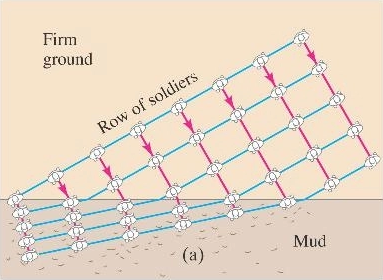
\includegraphics[width=.4\linewidth]{refraction_soldats.png}
    \caption{La réfraction d'une ligne de soldats.}
\end{figure}

\newpage

\subsection{Loi de la réfraction}
Lorsqu'une onde est réfractée en traversant une surface :
\(\frac{sin (\theta _i)}{v_i} = \frac{sin (\theta _r)}{v_r} \) où : \(v_i\) et \(v_r\) sont respectivement la vitesse de l'onde dans le milieu d'incidence et dans le milieu de réfraction.

\definecolor{qqccqq}{rgb}{0,0.8,0}
\definecolor{qqwuqq}{rgb}{0,0.39215686274509803,0}
\definecolor{qqqqff}{rgb}{0,0,1}
\definecolor{ffqqqq}{rgb}{1,0,0}
\definecolor{uuuuuu}{rgb}{0.26666666666666666,0.26666666666666666,0.26666666666666666}
\begin{tikzpicture}[line cap=round,line join=round,>=triangle 45,x=1cm,y=1cm]
    %\clip(-11.32,-9.62) rectangle (11.32,9.62);
    \draw [shift={(3,4)},line width=2pt,color=qqwuqq,fill=qqwuqq,fill opacity=0.10000000149011612] (0,0) -- (180:2) arc (180:220.8150838748816:2) -- cycle;
    \draw [shift={(3,4)},line width=2pt,color=qqwuqq,fill=qqwuqq,fill opacity=0.10000000149011612] (0,0) -- (0:2) arc (0:15.69198853284166:2) -- cycle;
    \draw [line width=2pt] (3,1)-- (3,7);
    \draw [line width=2pt,color=ffqqqq] (-0.96,0.58)-- (3,4);
    \draw [line width=2pt,color=ffqqqq] (1.1335234511653747,2.388042980551913) -- (1.1376515766622974,2.153771858601551);
    \draw [line width=2pt,color=ffqqqq] (1.1335234511653747,2.388042980551913) -- (0.9023484233377034,2.4262281413984486);
    \draw [line width=2pt,color=qqqqff] (3,4)-- (8.98,5.68);
    \draw [line width=2pt,color=qqqqff] (6.134409436118474,4.880569875029939) -- (6.038683850035927,4.666708676657833);
    \draw [line width=2pt,color=qqqqff] (6.134409436118474,4.880569875029939) -- (5.941316149964075,5.013291323342167);
    \draw [line width=2pt,color=qqccqq] (8.86,4)-- (-2.32,4);
    \begin{scriptsize}
        \draw[color=black] (3.4,4.23) node {\(f\)};
        \draw [fill=uuuuuu] (3,4) circle (2pt);
        \draw[color=uuuuuu] (3.16,4.39) node {\(C\)};
        \draw[color=ffqqqq] (1.3,2.29) node {\(i\)};
        \draw[color=qqqqff] (6.56,5.61) node {\(r\)};
        \draw[color=qqwuqq] (1.4,3.13) node {\(\theta _i\)};
        \draw[color=qqwuqq] (6.38,4.37) node {\(\theta _r\)};
        \draw[color=qqccqq] (1.74,4.59) node {\(n\)};
    \end{scriptsize}
\end{tikzpicture}

\subsection{Exercice}
La vitesse de propagation d'une onde sismique P traversant la frontière entre deux couches rocheuses augmente de 6,5 km/s à 8 km/s. Si l'angle d'incidence de l'onde avec la frontière est de \(30^{\circ}\), quel est l'angle de réfraction.

\subsection{Lumière et indice de réfraction}
La loi de Lenz s'applique évidement pour la lumière, cette dernière se comportant comme une onde. Dans le cas de la lumière, il existe une vitesse de référence : la vitesse dans le vide : \(c \approx 3 \times 10^8 [m/s]\). Il est donc plus commode de travailler avec un indice de réfraction : le rapport entre \(c\) et la vitesse de la lumière dans le milieu considéré : \(n_i=\frac{c}{v_i}\) . L'indice de réfraction varie en fonction de la longueur d'onde et des caractéristiques du milieu (matière, pression, température, \ldots).
\begin{itemize}
    \item Réécris la loi de Lenz en l'exprimant à partir des indices de réfraction des deux milieux traversés.
    \item Montre qu'un rayon lumineux passant successivement d'un milieu \enquote{1} vers un milieu \enquote{2} puis à nouveau vers le milieu \enquote{1} ressort parallèlement au rayon d'origine.
\end{itemize}

\newpage

\section{Diffraction des ondes}
Aussi longtemps qu'une onde ne change pas de milieu ou ne rencontre pas d'obstacle, elle se propage en ligne droite. En est-il de même si l'onde passe près de bords d'obstacle qui empêchent sa propagation ?

L'illustration \ref{fig:diffraction_I}, montre qu'une zone d'ombre se forme derrière un obstacle, mais qu'elle disparaît progressivement. L'illustration \ref{fig:diffraction_II}, montre que la zone d'ombre est d'autant plus grande que l'obstacle est grand.
Mais par rapport à quoi l'obstacle doit-il être grand ou petit ? C'est le rapport entre la largeur de celui-ci et la longueur d'onde qui détermine l'importance de l'ombre et on en déduit que les obstacles deviennent pratiquement \enquote{invisibles} lorsque leur taille est comparable ou inférieur à la longueur d'onde.

\begin{figure}[ht]
    \begin{minipage}{.5\textwidth}
        \centering
        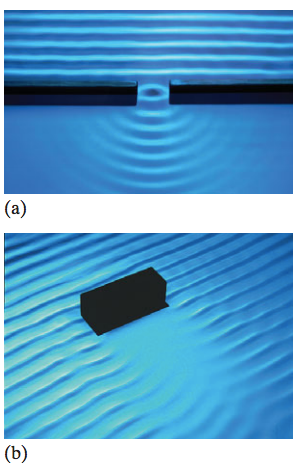
\includegraphics[width=.8 \linewidth]{diffraction_I.png}
        \caption{Diffraction des ondes.}
        \label{fig:diffraction_I}
    \end{minipage}
    \begin{minipage}{.5\textwidth}
        \centering
        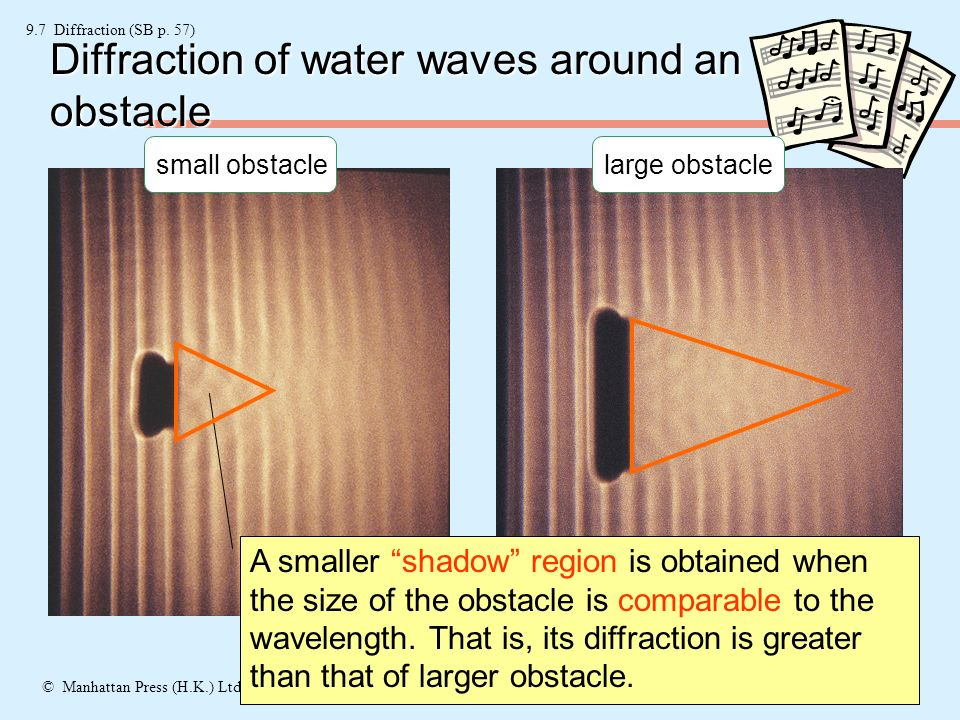
\includegraphics[width=.8 \linewidth]{diffraction_II.png}
        \caption{Taille de la zone d'ombre en fonction de la taille de l'obstacle.}
        \label{fig:diffraction_II}
    \end{minipage}
\end{figure}

\newpage

\subsection{Comprendre la diffraction : principe de Huygens}
Le principe de Huygens est simple et un lien clair peut être fait avec la résonance des oscillateurs :
\begin{encadre}
    \motcle{Principe de Huygens} : Lorsqu'une onde se propage, chaque élément de surface atteint par cette onde, se comporte comme une source secondaire qui émet des ondelettes sphériques appelées ondelettes d'Huygens.
\end{encadre}
L'oeil ne distingue pas ces ondelettes, mais uniquement leur enveloppe. Le front de l'onde à un instant \(t+\delta t\) se déduit du front de cette onde à l'instant \(t\), en considérant que l'enveloppe des ondes secondaires d'Huygens s'est propagée pendant l'intervalle de temps \(\delta t\), comme le montre la figure ci-dessous.

\begin{figure}[ht]
    \centering
    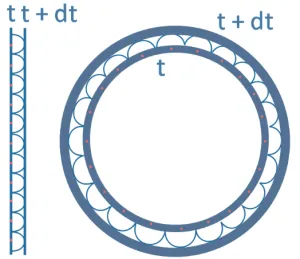
\includegraphics[width=.4\linewidth]{principe_huygens.png}
    \caption{Principe de Huygens (illustration et commentaire de \enquote{osez-reussir-en-physique.com})}
\end{figure}

Chaque point de part et d'autre d'un obstacle se comporte comme une source ponctuelle et un front d'onde se reforme dès lors derrière ceux-ci.
Lorsqu'une onde rencontre un obstacle complet comportant une fente étroite, celle-ci se comporte comme une source d'onde circulaire, ce phénomène est clairement visible dans l'illustration \ref{fig:diffraction_I} a et l'illustration \ref{fig:diffraction_IV}.

\begin{figure}[ht]
    \begin{minipage}{.5\textwidth}
        \centering
        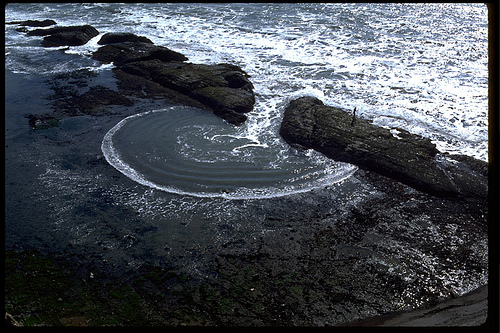
\includegraphics[width=.8\linewidth]{diffraction_IV.png}
        \caption{La diffraction à travers une fente étroite.}
        \label{fig:diffraction_IV}
    \end{minipage}
    \begin{minipage}{.5\textwidth}
        \centering
        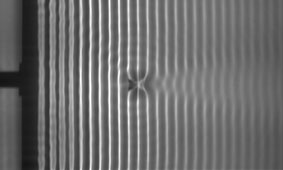
\includegraphics[width=.8\linewidth]{diffraction_III.png}
        \caption{La diffraction autour d'un obstacle de petite taille.}
        \label{fig:diffraction_III}
    \end{minipage}
\end{figure}

\subsection{Applications}

\begin{tcolorbox}[title=Ondes acoustiques]
    Le son est une onde dont la fréquence est comprise entre 20 Hz (fréquence la plus grave) et 20 000 Hz (fréquence la plus aiguë). La fréquence de référence est la note \enquote{la} (\(f=440[Hz]\)) à laquelle correspond une longueur d'onde de \(\lambda=0,77[m]\). Une longueur d'onde de \(1 [m]\) est associée aux sons de \(340[Hz]\). On réalise que les objets du quotidien (table, chaise, armoire, ouverture de porte, \ldots) permettent une bonne diffraction des sons, c'est la raison pour laquelle ils se propagent bien dans l'ensemble des espaces que nous occupons.
\end{tcolorbox}

\begin{tcolorbox}[title=Écholocation]
    Lorsque les ondes diffractent bien autour d'un objet, elles s'y réfléchissent peu. La perception d'un corps grâce aux ondes qui s'y réfléchissent comme dans le cas du sonar, de l'écholocation (ondes sonores) ou du radar (ondes électromagnétiques) n'est donc possible que si la taille de l'objet recherché est plus grande que la longueur d'onde utilisée.
    La voix humaine crée en moyenne des ondes sonores comprises entre 125 et 210 Hertz, tandis qu'une chauve-souris génère des ondes comprises entre 15 000 et 150 000 Hz. Cet animal se nourri essentiellement d'insectes, comme les moustiques dont la taille est entre 0,5 et 1,5 centimètres.
    \begin{itemize}
        \item Calcule la taille des corps perceptibles par une chauve-souris. Cela correspond-il à celle des insectes dont elles se nourrissent ?
    \end{itemize}
\end{tcolorbox}



\begin{tcolorbox}[title=Sonar]
    La fréquence d'émission d'un sonar est choisie en fonction de son utilisation. Les hautes fréquences (plusieurs dizaines ou centaines de kHz) sont rapidement absorbées par l'eau de mer (plusieurs centaines de mètres) mais, en revanche, permettent la détection de petits objets et peuvent ainsi réaliser de véritables images. Employées à une fréquence de 14 à 22 kilohertz durant la Seconde Guerre mondiale, elles sont donc, depuis, utilisées pour les sondeurs hydrographiques, les sonars de pêche, pour la recherche de mines, pour la détection de torpilles.
    Plus on descend en fréquence, plus les distances de détection sont grandes, mais on perd en finesse et les antennes deviennent très grandes et très lourdes. En pratique, les sonars actifs très basse fréquence ne descendent guère en dessous de 3 kHz. Les portées de détection n'excèdent pas quelques dizaines de kilomètres.
\end{tcolorbox}

\begin{figure}[ht]
    \begin{minipage}{.5\textwidth}
        \centering
        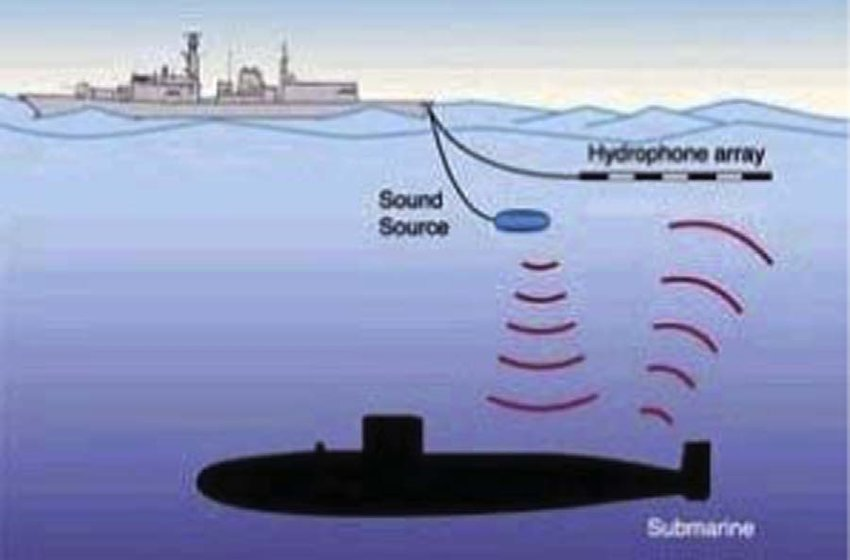
\includegraphics[width=.8\linewidth]{sonar.png}
        \caption{Le sonar}
    \end{minipage}
    \begin{minipage}{.5\textwidth}
        \centering
        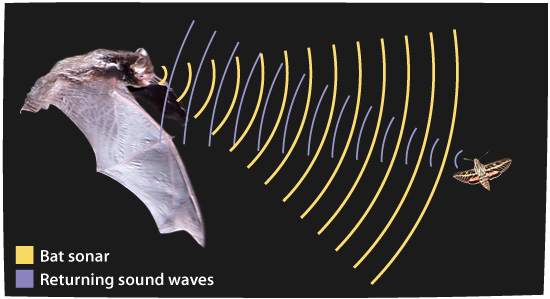
\includegraphics[width=.8\linewidth]{echolocation.png}
        \caption{L'écholocation chez les chauves-souris.}
    \end{minipage}
\end{figure}

\newpage

\section{Interférences}
Quand deux ondes atteignent simultanément un même point, elles vont agir dessus en respectant le \motcle{principe de superposition}. Si ces deux ondes sont de même amplitude, mais en opposition de phase, elles vont s'annuler mutuellement, on parle dans ce cas d'\motcle{interférences destructives}.
Si, au contraire, elles sont de même amplitude et en concordance de phase, elles vont se combiner et créer une \motcle{interférence constructive}.

\begin{figure}[ht]
    \centering
    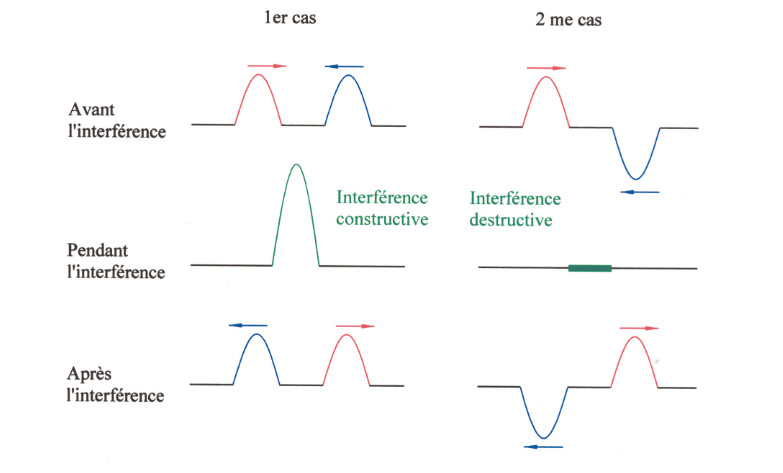
\includegraphics[width=.8\linewidth]{interference.png}
    \caption{Interférences constructives et destructives}
\end{figure}

\newpage

\section{Interférences entre deux sources ponctuelles}
Lorsque deux sources \textbf{en phase} et de \textbf{même amplitude} font vibrer le même milieu, chaque point de ce milieu va être affecté par les deux signaux. Il va donc y avoir une interférence des deux signaux en chaque point et une \motcle{figure d'interférence} va apparaître sur l'ensemble du milieu.

\begin{figure}[ht]
    \centering
    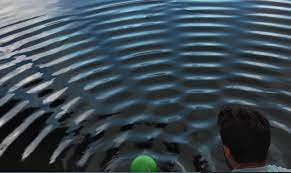
\includegraphics[width=\linewidth]{interference_deux_sources.png}
    \caption{Figure d'interférence pour deux sources en phase à la surface de l'eau.}
\end{figure}

\newpage

La figure ci-dessous représente un milieu soumis à l'influence de deux sources ponctuelles, en phase et de même amplitude. Repère sur cette figure les points correspondant aux interférences constructives et aux interférences destructives. Relie entre eux les points d'interférence constructive de manière à mettre en évidence les \motcle{lignes de tempête}, fais de même avec les interférences destructives pour mettre en évidence les \motcle{lignes de repos}.

\hfill \break

\begin{tikzpicture}[]
    \tkzDefPoints{-2/0/S1,2.5/0/S1_1UP,1.5/0/S1_2UP,2/0/S1_1DOWN,1/0/S1_2DOWN}
    \tkzDrawCircle[color=blue](S1,S1_1UP)
    \tkzDrawCircle[color=blue](S1,S1_2UP)
    \tkzDrawCircle[color=blue,style=dashed](S1,S1_1DOWN)
    \tkzDrawCircle[color=blue,style=dashed](S1,S1_2DOWN)

    \tkzDefPoints{2/0/S2,-2.5/0/S2_1UP,-1.5/0/S2_2UP,-2/0/S2_1DOWN,-1/0/S2_2DOWN}
    \tkzDrawCircle[color=red](S2,S2_1UP)
    \tkzDrawCircle[color=red](S2,S2_2UP)
    \tkzDrawCircle[color=red,style=dashed](S2,S2_1DOWN)
    \tkzDrawCircle[color=red,style=dashed](S2,S2_2DOWN)

    \tkzDrawPoint[color=blue,size=4pt](S1)
    \tkzDrawPoint[color=red,size=4pt](S2)
    \tkzLabelPoint(S1){\(S_1\)}
    \tkzLabelPoint(S2){\(S_2\)}

\end{tikzpicture}

\newpage

\begin{figure}[ht]
    \centering
    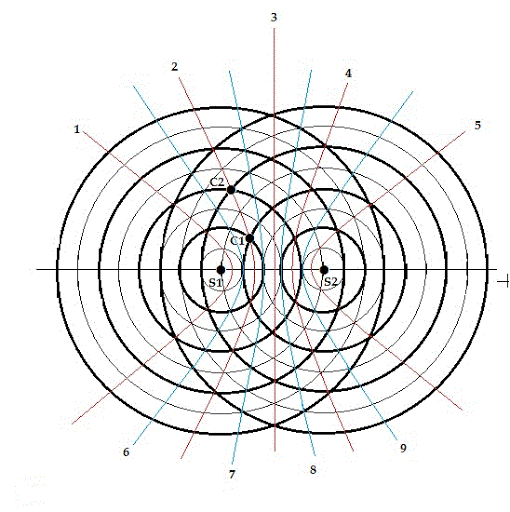
\includegraphics[width=\linewidth]{figure_interference.png}
    \caption{Figure d'interférence avec les lignes de tempête et de repos.}
\end{figure}

\newpage

\subsection{Condition d'interférences constructives ou destructives}
Dans la figure ci-dessous, les points rouges correspondent à des interférences constructives.
\begin{itemize}[label=\textbullet]
    \item Pour quelle raison y a-t-il des interférences constructives en ces points ?
          \pointilles{3}
\end{itemize}

\begin{figure}[ht]
    \centering
    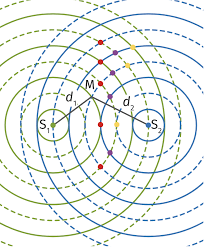
\includegraphics[width=.4\linewidth]{figure_interference_II.png}
    \caption{Figure d'interférence pour deux sources en phase.}
\end{figure}

La \motcle{différence de marche}, \(\lambda\), en un point correspond à la différence de distance entre ce point et chacune des deux sources : \(\delta _M=d_2 - d_1\). On peut donc dire qu'il y a une interférence constructive si la différence de marche vaut 0, mais ce n'est pas suffisant. En effet, il existe d'autres points présentant une interférence constructive, mais pour lesquels \(\delta \neq 0\), les points jaunes par exemple.

\newpage

\begin{itemize}[label=\textbullet]
    \item Quel doit être le déphasage entre les deux signaux arrivant sur un point jaune pour qu'ils interfèrent de manière deconstructive ?
          \pointilles{2}
    \item Que doit valoir la différence de marche en un point pour qu'il y ait une interférence constructive ?
          \pointilles{2}
\end{itemize}



Par un raisonnement similaire, on comprend qu'un point subit des interférences destructives si les signaux qui lui parviennent sont en opposition de phase, ce qui implique que la différence de marche vaut :

\begin{encadre}
    \motcle{Interférence destructive} : \(\delta = (2k+1) \frac{\lambda}{2} \ \ (k=0,1,2,3,...)\)
\end{encadre}

\begin{encadre}
    \motcle{Interférence constructive} : \(\delta = k \lambda \ \ (k=0,1,2,3,...)\)
\end{encadre}

\newpage

\begin{figure}[ht!]
    \centering
    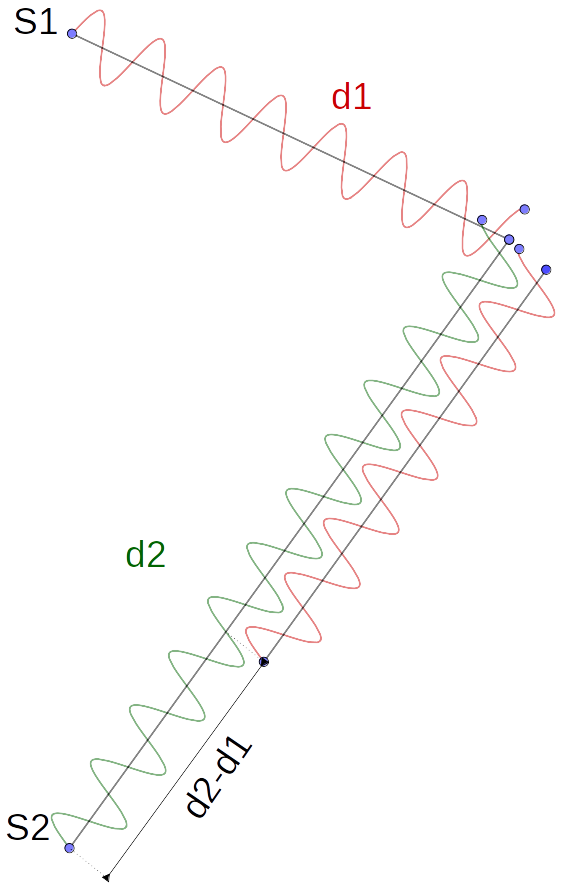
\includegraphics[width=.8\linewidth]{interference_difference_marche.png}
    \caption{La différence de marche vaut 4 lambda.}
\end{figure}

\newpage

\subsection{Étude mathématique des interférences}
Nous avons vu que l'élongation d'un point en fonction de sa distance à la source (\(x\)) et en fonction du temps (\(t\)) est donnée par : \(y_P (t) = A \cdot sin (\omega \cdot t- \frac{2 \pi  \cdot x}{\lambda})\).
Si un point se trouve à une distance \(x_1\) de la source \(S_1\) et une distance \(x_2\) de la source \(S_2\), alors, en vertu du principe de superposition, son élongation totale est donnée par :
\begin{equation}
    y_P (t) = A \cdot sin (\omega \cdot t- \frac{2 \pi  \cdot x_1}{\lambda}) + A \cdot sin (\omega \cdot t- \frac{2 \pi  \cdot x_2}{\lambda})
\end{equation}

On peut mettre l'amplitude en évidence pour avoir :
\begin{equation}
    y_P (t) = A \left \lbrace \cdot sin (\omega  \cdot t- \frac{2 \pi  \cdot x_1}{\lambda}) +  \cdot sin (\omega \cdot t- \frac{2 \pi  \cdot x_2}{\lambda}) \right \rbrace
\end{equation}

On sait que \(sin( a) + sin (b)=2 \cdot sin( \frac{a+b}{2}) \cdot cos(\frac{a-b}{2})\), donc :

\begin{equation}
    y_P (t) = A \cdot  sin \left \lbrace (\omega  \cdot t)- \frac{ \pi  \cdot (x_1+x_2)}{\lambda} \right \rbrace   \cdot cos \left \lbrace \frac{\pi}{\lambda}\cdot (x_1-x_2) \right \rbrace
\end{equation}

Cette équation est exactement celle de l'élongation d'un point dans le temps et dans l'espace, mais pour laquelle l'amplitude vaut \(A \cdot cos (\frac{\pi}{\lambda}\cdot (x_1-x_2) )\).

\subsubsection{Interférences destructives}
On sait que cette amplitude vaut \(0\) si \(cos \left \lbrace \frac{\pi}{\lambda}\cdot (x_1-x_2) \right \rbrace = 0\) , donc si :
\begin{equation}
    \frac{\pi}{\lambda}\cdot (x_1-x_2) = \frac{\pi}{2}+k \cdot \pi
\end{equation}

Ce qui revient à dire :
\begin{equation}
    (x_1-x_2) = \frac{\lambda}{2} \cdot (1+2\cdot k )
\end{equation}
Cette dernière équation correspond exactement à la condition pour laquelle il y a une interférence destructive.

\subsubsection{Interférences constructives}
En utilisant le même raisonnement, retrouve la condition de formation des interférences constructives.

\newpage

\section{Exercices}
\begin{exercise}
    Deux haut-parleurs sont distants de 1m et émettent un son à 1150Hz à une température de \(20^\circ C\). Une personne se trouve à 4m de l'un des hauts-parleurs, à quelle distance doit-elle se trouver du deuxième pour percevoir une interférence destructive ?
\end{exercise}
\begin{solution}\\
    \(k=1 \rightarrow x_2=4,296[m]\)\\
    \(k=-1 \rightarrow x_2=3,704[m]\)\\
    La deuxième réponse est \enquote{plus intéressante}, mais les deux sont acceptées.
\end{solution}

\begin{exercise}
    Deux haut-parleurs S1 et S2 distants de 6m émettent des ondes sonores en phase. Un point P se trouve à une distance de 8m de S1.
    \begin{enumerate}[a)]
        \item Pour quelle fréquence l'intensité en P est-elle maximale ?
        \item Pour quelle fréquence l'intensité en P est-elle minimale ?
    \end{enumerate}
    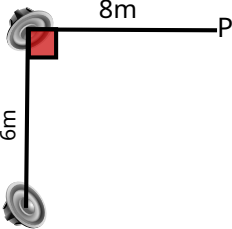
\includegraphics[width=.2\linewidth]{exercice_hauts_parleurs.png}
\end{exercise}
\begin{solution}
    \begin{enumerate}[a)]
        \item \(f=125,53[Hz]\)
        \item \(f=62,765[Hz]\)
    \end{enumerate}
\end{solution}

\begin{exercise}
    Deux haut-parleurs sont distants de 2,5m dans un local à \(20 ^ \circ C\). Une personne se tient à 3m de l'un des haut-parleurs et 3,5m de l'autre.
    \begin{enumerate}[a)]
        \item Quelle est la fréquence minimale qui provoque une interférence destructive en ce point ?
        \item Trouve deux autres fréquences qui provoque ce phénomène.
    \end{enumerate}
\end{exercise}
\begin{solution}
    \begin{enumerate}[a)]
        \item \(f_1=340[Hz]\)
        \item \(f_2=1020[Hz] ; f_3=1700[Hz]\)
    \end{enumerate}
    \(f_2\) et \(f_3\) correspondent à \(3 \cdot f_1\) et \(5 \cdot f_1\) puisque les interférences destructives sont obtenues avec les entiers impairs.
\end{solution}


\begin{exercise}
    Dans un local à \(20 ^\circ C\), une personne entend un son pur provenant de deux sources en phase et de même fréquence. Celle-ci est comprise entre 500 et 1000Hz. Le volume le plus élevé se trouve au point équidistant des deux sources. Afin de déterminer exactement la fréquence des sources, la personne se déplace et constate que le niveau est minimal lorsqu'elle est plus proche de 0,22m d'une des deux sources. Quelle est la fréquence du son ?
\end{exercise}
\begin{solution}
    Dans cette situation, on sait que : \(f=(2k+1) \cdot 772,727\).
    Pour \(k=1\), \(f=772,727[Hz]\). Cette fréquence est bien comprise entre 500 et 1000[Hz].
\end{solution}
\chapter{Les ondes stationnaires}
Lorsqu'une impulsion unique, une onde simple, est envoyée sur une corde fixée à ses deux extrémités, elle va se réfléchir et revenir \enquote{inversée} c'est-à-dire avec la même élongation, mais une vitesse opposée. Si, au lieu d'une onde unique, on envoie une onde continue (voir \ref{Onde unique et onde entretenue}), les ondes réfléchies vont interférer avec les ondes directes et l'ensemble va présenter un profil complexe.

Toutefois, si la fréquence est choisie de manière adéquate par rapport à la vitesse de l'onde et la longueur de la corde, il est possible de créer une \motcle{onde stationnaire} : une situation dans laquelle les ondes réfléchies interfèrent constructivement avec les ondes directes à certains endroits et destructivement à d'autres.


Les points d'interférence destructive, qui sont donc immobiles sont appelés \motcle{noeuds}. Les points d'interférence constructive sont appelés \motcle{anti-noeuds} ou \motcle{ventres}.
La plus petite fréquence permettant d'obtenir une onde stationnaire donne un profil tel qu'illustré ci-dessous :

\begin{figure}[h!]
    \centering
    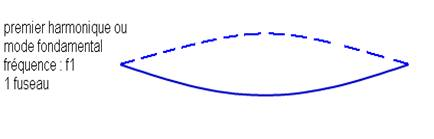
\includegraphics[width=.8\linewidth]{onde_stationnaire_fond1.png}
    \caption{Mode fondamentale d'une onde stationnaire : un ventre, deux nœuds.}
\end{figure}

Le profil de l'onde correspond à : \(L=\frac{\lambda}{2}\) où L est la longueur de la corde. La fréquence associée est : \(f=\frac{v}{2 \cdot L}\). Cette première onde stationnaire est appelée \motcle{première harmonique} ou \motcle{fondamentale}.

La deuxième fréquence permettant d'obtenir une onde stationnaire donne le profil ci-dessous :
\begin{figure}[h!]
    \centering
    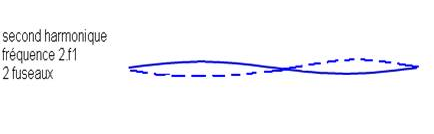
\includegraphics[width=.8\linewidth]{onde_stationnaire_harm2.png}
    \caption{Deuxième harmonique : deux ventres, trois nœuds.}
\end{figure}

Le profil de l'onde correspond à : \(L=2 \cdot \frac{\lambda}{2}\). La fréquence associée est : \(f=\frac{v}{ L}\). Cette deuxième onde stationnaire est appelée \motcle{deuxième harmonique}.

La troisième harmonique est associée au profil ci-dessous, pour lequel  \(L=3 \cdot \frac{\lambda}{2}\).
\begin{figure}[h!]
    \centering
    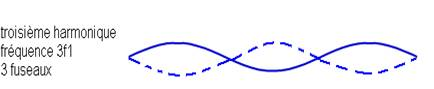
\includegraphics[width=.8\linewidth]{onde_stationnaire_harm3.png}
    \caption{Troisième harmonique : trois ventres, quatre nœuds.}
\end{figure}

Si on généralise, on voit que les différentes ondes stationnaires qui peuvent prendre place sur une corde de longueur \(L\) avec les deux extrémités fixes correspondent à  \(L=k \cdot \frac{\lambda}{2}\) et que les fréquences associées valent :
\begin{equation}
    f=k \cdot \frac{v}{2 \cdot L}
\end{equation}

Au cours de la séance de labo sur les ondes stationnaires, nous avons vu que la vitesse d'une onde sur une corde dépend de la tension dans la corde, \(F_T\), et de la masse linéique, \(\mu\). La relation utilisée était : \(v=\sqrt{\frac{F_T}{\mu}}\). Si on combine les deux relations, on constate que les fréquences permettant l'obtention d'une onde stationnaire sur une corde soumise à une tension \(F_T\) et d'une masse linéique \(\mu\) s'obtiennent par :
\begin{equation}
    f=k \cdot \sqrt{\frac{F_T}{4\cdot \mu \cdot L^2}}
\end{equation}

Selon la valeur de \(k\), on obtient la première, la deuxième, la troisième, … harmonique.

\newpage

\section{Application : instrument à corde}
Lorsqu'on pince une corde de guitare, des ondes de fréquences très variées sont générées. La plupart de ces ondes disparaissent rapidement, mais les ondes stationnaires persistent. Il n'y a pas qu'une harmonique qui persiste, mais une combinaison de différentes harmoniques.

La longueur de la corde est fixée par celle du manche (distance entre le point d'attache et l'extrémité du manche), les clés permettent de régler la tension et le type de corde détermine la masse linéique.
Lorsque le joueur produit un \(La\), la corde vibre simultanément à différentes harmoniques.

Puisque la corde est fixée à ses deux extrémités, les harmoniques sont des multiples entiers les unes des autres : 220, 440, 660, … [Hz]. C'est la proportion des différentes harmoniques qui constitue le son propre, le \motcle{timbre}, du \(La\) sur une  guitare et qui le distingue de la même note sur un autre instrument.

\begin{figure}[h!]
    \centering
    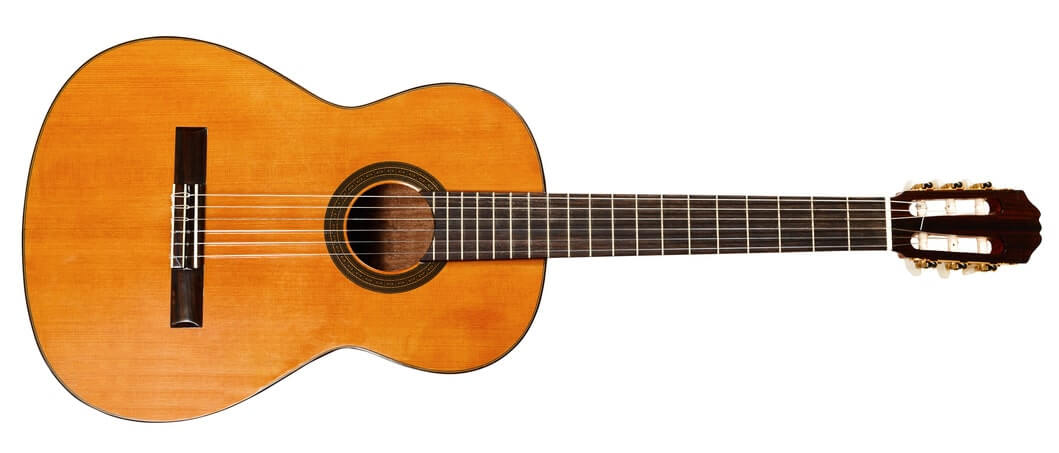
\includegraphics[width=.5\linewidth]{guitare.png}
    \caption{Une guitare}
\end{figure}

\newpage

\begin{figure}[h!]
    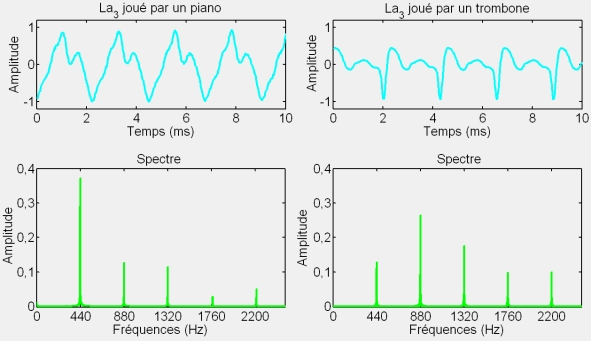
\includegraphics[width=.8\linewidth]{spectre_sonore.png}
    \caption{Le spectre sonore d'un trombone et d'un piano pour la note La. C'est le spectre qui détermine le timbre.}
\end{figure}

\begin{figure}[h!]
    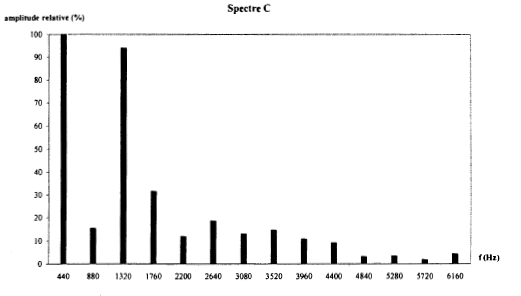
\includegraphics[width=.8\linewidth]{spectre_guitare_la.png}
    \caption{Le spectre d'une guitare pour la note La}
\end{figure}

\newpage

\section{Exercices}
\begin{exercise}
    La longueur et la masse d'une corde de piano sont respectivement de 1,1m et de 9,00 g.
    \begin{enumerate}[a)]
        \item Quelle doit être la tension dans la corde pour qu'elle vibre à une fréquence fondamentale de 131 Hz (Do, octave 3) ?
        \item Quelles sont les fréquences des quatre premières harmoniques ?
    \end{enumerate}
\end{exercise}
\begin{solution}
    \(F_T=679,58[N]\)
\end{solution}

\begin{exercise}
    Un ukulélé \enquote{concert} a une longueur de corde d'environ 40cm, tandis qu'une guitare à une longueur de 64cm. On souhaite produire la même fondamentale sur ces deux instruments. Si on place la même corde sur les deux instruments, laquelle doit être la plus \enquote{tendue} ? Quel est le rapport entre les deux tensions ?
    \begin{figure}[h!]
        \centering
        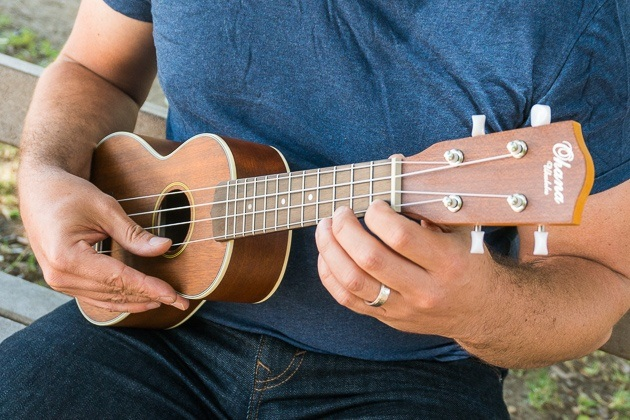
\includegraphics[width=.4\linewidth]{ukulele.png}
        \caption{Un ukulélé}
    \end{figure}
\end{exercise}
\begin{solution}
    Dans cette situation, \(\mu\) est identique pour les deux instruments puisqu'il s'agit de la même corde. Donc :
    \(\frac{F_{T1}}{L_1 ^2}=\frac{F_{T2}}{L_2 ^2}\) \\
    Si on remplace \(L_1\) et \(L_2\) par leurs valeurs respectives, on obtient :\\
    \(F_{T1}=0,3906 \cdot F_{T2}\) .\\
    \(F_{T1}\) est donc plus petit que \(F_{T2}\), la deuxième corde est plus tendue que la première. Le rapport entre les deux tensions est de \(0,3906\).
\end{solution}


\begin{exercise}
    Une corde de violon vibre à 440[Hz] lorsqu'on la relâche après l'avoir pincée. À quelle fréquence vibre-t-elle si on la pince après avoir diminué sa longueur de 25\% ?
\end{exercise}
\newpage
\begin{solution}
    \begin{equation*}
        \begin{aligned}
            f_1                   & =\sqrt{\frac{F_T}{4 \mu L_1 ^2}}                                               \\
            f_2                   & =\sqrt{\frac{F_T}{4 \mu (0,75 L_1)^2}}                                         \\
            \frac{f_1}{f_2}       & =\frac{\sqrt{\frac{F_T}{4 \mu L_1 ^2}}}{\sqrt{\frac{F_T}{4 \mu (0,75 L_1)^2}}} \\
            \frac{f_1 ^2}{f_2 ^2} & =\frac{F_T}{4 \mu L_1 ^2}  \cdot \frac{4 \mu (0,75 L_1)^2}{F_T}                \\
            \frac{f_1}{f_2}       & =\frac{3}{4}                                                                   \\
            f_2                   & =\frac{4}{3} \cdot f_1                                                         \\
            f_2                   & =586,67[Hz]
        \end{aligned}
    \end{equation*}

\end{solution}

\begin{exercise}
    La vitesse des ondes sur une corde de 5,496 [m] est de 480 m/s. Un régime stationnaire est obtenu si la fréquence est de 131[Hz].
    \begin{enumerate}[a)]
        \item Combien de noeuds y'a-t-il ?
        \item À quelle distance les uns des autres se trouvent les noeuds ?
    \end{enumerate}
\end{exercise}
\begin{solution}
    \begin{enumerate}[a)]
        \item Il y a 4 noeuds.
        \item La distance entre deux noeuds est de \(\frac{\lambda}{2}\), donc : \(d=1,8321[m]\)
    \end{enumerate}
\end{solution}

\begin{exercise}
    On attache une corde horizontale d'une masse linéique de \(4,2 \times 10^{-4} [kg \cdot m^{-1}]\) par l'une de ses extrémités à un vibrateur oscillant à 60[Hz] avec une faible amplitude. La corde passe par une poulie située à une distance \(L=1,4[m]\) de l'extrémité fixée au vibrateur et des poids sont suspendus à l'autre extrémité.
    Quelle doit être la masse suspendue à l'extrémité de la corde pour produire 5 ventres ? On considère que l'extrémité fixée au vibrateur correspond à un noeud, car l'amplitude du signal est faible par rapport à celle des interférences.
\end{exercise}
\begin{solution}
    On sait que : \(F_T=\frac{f^2 \cdot 4 \cdot \mu \cdot L^2}{k^2}\). \\
    Dans cette situation, \(k=5\) puisqu'on veut obtenir 5 ventres. Donc :\\
    \(F_T=0,4742[N]\) \\
    \(m=0,04833[kg]\)

\end{solution}
\tableofcontents
\newpage
\printallsolutions
\end{document}
